\documentclass[cs4size, twoside, fancyhdr, fleqn, openany, hyperref]{ctexbook}

% Import the packages
\usepackage[]{graphicx} % For the insertion of the graphs
\usepackage{float} % For detailed control of the float
\usepackage[tbtags]{amsmath} % For math op
\usepackage{amssymb} % For math op
% \usepackage{upgreek} % For math op
\usepackage{bbm} % For \mathbbm{1}
\usepackage{mathtools} % For math op
\usepackage{geometry} % For the style of the geometry
\usepackage[font=small, labelfont=bf]{caption} % For the style of the caption
\usepackage[nottoc]{tocbibind}
% \usepackage[normalem]{ulem}
\usepackage{enumitem}
\usepackage{latexsym}
\usepackage[perpage]{footmisc} % For more control on page foot
\usepackage{tocloft}
\usepackage[pdfborder={0 0 0}]{hyperref} % For links in pdf
\usepackage[style=authoryear-comp, natbib]{biblatex}
% \usepackage{makeidx}
% \usepackage{glossaries}
\usepackage{color} % For color support
\usepackage{xcolor} % For color support
\usepackage{longtable} % For longtable environment
\usepackage{wrapfig} % For wrapfigure environment
\usepackage[many]{tcolorbox} % For tcolorbox environment
\usepackage{expl3} % For \Repeat macro
\usepackage[section]{placeins} % For \FloatBarrier macro
\usepackage{pdfpages} % For the insertion of the cover image

% Set the style of the book
\geometry{a4paper, centering, scale=0.8}
\punctstyle{kaiming}
\linespread{1.4}
\ctexset{chapter={number={\arabic{chapter}}, format+={\raggedright}, aftername={\\}}, section={name={,节}, format+={\raggedright}}}
\pagestyle{fancy}
\fancyhf{}
\fancyhead[LO]{\slshape \rightmark}
\fancyhead[RE]{\slshape \leftmark}
\fancyhead[LE, RO]{\thepage}
\newlength{\ecgluelen}
\setlength{\ecgluelen}{2.3pt plus .3pt minus .1pt}
%\CJKsetecglue{\hspace{\ecgluelen}}

% Set the format of the ref
\newcommand{\refglue}{\hspace{\ecgluelen}}
\newcommand{\partref}[1]{\hyperref[part:#1]{第\zhnumber{#1}部分}}
\newcommand{\chapref}[1]{\hyperref[chap:#1]{第\refglue #1\refglue 章}}
\newcommand{\secref}[1]{\hyperref[sec:#1]{\refglue #1\refglue 节}}
\newcommand{\figref}[1]{\hyperref[fig:#1]{图\refglue #1\refglue}}
\newcommand{\examref}[1]{\hyperlink{exam:#1}{例\refglue #1\refglue}}

% Set the the depth
\setcounter{secnumdepth}{2}
\setcounter{tocdepth}{2}

% Add the bib file
\addbibresource{rl-cn.bib}

% Set the title of the book
\title{强化学习导论}
\author{Richard S. Sutton \and Andrew G. Barto}
\CTEXoptions[today=small]
\date{\today}

% Define math operators
\DeclareMathOperator{\targmax}{argmax}
\DeclareMathOperator*{\dargmax}{argmax}

\DeclareMathAlphabet{\mathpzc}{OT1}{pzc}{m}{it}

% Define exercise environment
\newcounter{exercnt}[chapter]
\renewcommand{\theexercnt}{\arabic{chapter}.\arabic{exercnt}}
\newenvironment{exer}[1][]{%
	\par\noindent\stepcounter{exercnt}\textit{练习 \theexercnt: #1}\quad%
}%
{%
	\mbox{}~\hfill $\Box$%
}

% Define example environment
\newcounter{examcnt}[chapter]
\renewcommand{\theexamcnt}{\arabic{chapter}.\arabic{examcnt}}
\newenvironment{exam}[1][]{%
	\par\noindent\stepcounter{examcnt}\textit{例 \theexamcnt: #1}\quad%
}%
{%
	\mbox{}~\hfill $\blacksquare$%
}

% Define pcbox environment(used to contain pseudocode)
\ExplSyntaxOn
\cs_new_eq:NN \Repeat \prg_replicate:nn
\ExplSyntaxOff
\newcommand{\pcind}[1][1]{\Repeat{#1}{\phantom{m}}}
\newenvironment{pcbox}[2]%
{%
	\par\noindent\begin{tcolorbox}[title={#1}, floatplacement=#2, float]%
}%
{%
	\end{tcolorbox}%
}

% Define mathbox environment(used to contain mathematical material)
\definecolor{framecolor}{rgb}{0.55, 0.55, 0.55}
\definecolor{bkcolor}{rgb}{0.95, 0.95, 0.95}
\definecolor{titlecolor}{rgb}{0.5, 0.5, 0.5}

\newenvironment{mathbox}[1]%
{%
	\par\noindent\begin{tcolorbox}[title={#1}, breakable, enhanced jigsaw, colframe=framecolor, colback=bkcolor, coltitle=titlecolor, colbacktitle=bkcolor, before=\vspace{1em}, before upper={\parindent2\ccwd}]%
}%
{%
	\end{tcolorbox}%
}

% Define flushing operation in math mode
\makeatletter
\newcommand{\pushright}[1]{\ifmeasuring@#1\else\omit\hfill$\displaystyle#1$\fi\ignorespaces}
\newcommand{\pushleft}[1]{\ifmeasuring@#1\else\omit$\displaystyle#1$\hfill\fi\ignorespaces}
\makeatother

\makeatletter
\newcommand{\specialcell}[1]{\ifmeasuring@#1\else\omit$\displaystyle#1$\ignorespaces\fi}
\makeatother

% Include the tex src files
\includeonly{c0/frontmatter, c1/introduction, c2/multi-armed_bandits, c3/finite_MDPs}
%\includeonly{c3/finite_MDPs} 

%---------------------------- The content of the book -------------------------------
\begin{document}
\frontmatter
\pagestyle{empty}

% Make the title
\begin{titlepage}
%\maketitle

\includepdf{c0/img/cover.pdf}
\cleardoublepage
\end{titlepage}

% Make the toc
\tableofcontents
\cleardoublepage

\pagestyle{fancy}

% Include front matter
%--------------------------- pautoreface 2 ---------------------------------
\phantomsection
\addcontentsline{toc}{section}{第2版序}
\section*{第2版序}\label{sec:pautoreface_2}

由本书的第一版出版至今的二十年见证了人工智能领域的巨大进步, 该进步很大程度上是由机器学习的发展推动的, 而机器学习的发展中也包括了强化学习的发展. 虽然计算能力的增强为这些发展中一部分做出了贡献, 但理论与算法上的新进展同样是强大的驱动力. 面对这样的进步, 相较于1998年版本的再版刻不容缓, 于是我们终于在2012年开始了这个项目. 本书第二版的目标同第一版是一致的: 向所有关联领域的读者, 提供清晰明了的强化学习关键概念与算法. 本版本依然是导论性质的, 并且我们仍将注意力集中于核心的在线<online>学习算法. 本版本包含了一些在间隔的这些年中重要性日渐凸显出来的主题, 并且我们拓宽了对我们现在理解得更好的主题的涵盖. 但我们不会试图提供对强化学习领域全面的覆盖, 因为其在许多不同的方向上有爆炸式的发展. 我们为不得不遗漏这些发展中的大部分而只能保留小部分而道歉.

就像在第一版中做的那样, 我们选择不以严密、正式的方式对强化学习进行阐述, 也不在最一般的情形下进行阐述. 然而, 自第一版以来我们在一些主题上形成了的更为深入的理解, 这些理解需要稍多的数学来解释; 我们将需要更多数学知识的部分用带阴影的方框隔开, 以便苦于数学的读者可以选择跳过. 我们也使用了和第一版略微不同的数学标记. 在教学的过程中, 我们发现新的标记系统可以解决一些普遍的疑惑. 这套标记系统强调了随机变量与其实例的区别, 其中前者标记为大写字母, 后者标记为小写字母. 举个例子, 时步$t$中的状态<state>, 动作<action>与奖赏<reward>分别被记为$S_t$, $A_t$与$R_t$,而它们可能的取值可以被记为$s$, $a$, $r$. 类似地, 可以很自然地将小写字母用于值函数<value function>(比如$v_{\pi}$), 并将大写字母限定于它们表格式<tabular>的估计值.  近似值函数<approximate value function>是任意参数的确定性<deterministic>函数, 因此也使用小写字母标记(例如$\hat v (\mathbf s, \mathbf w_t) \approx v_\pi(\mathbf s)$). 向量, 例如权重向量$\mathbf w_t$(或更为正式的${\boldsymbol \theta}_t$)以及特征向量$\mathbf x_t$(或更为正式的$\boldsymbol \phi_t$), 都是用粗体的小写字母标记, 即使它们为随机变量. 大写的粗体为矩阵保留. 在第一版中我们使用特定的标记$\mathfrak P_{s, s^\prime}^a$和$\mathfrak R_{s, s^\prime}^a$来分别标识转移概率与奖赏的期望值. 这两个标记的一个缺点是其仍然不能完全描述奖励的动态<dynamics>, 因为其只给出了奖励的期望值: 这对动态规划<dynamic programming>而言是足够了, 但对强化学习而言远远不够. 这两个标记的另一个缺点是对下标与上标的滥用. 在本版中我们使用$p(s', r \mid s, a)$这一明确的标记来表示给定当前状态与动作的情况下, 下一状态与奖赏的联合概率. 所有标识的变化都列于\hyperlink{sec:notation}{标识一览}中.

本版有了极大的拓展, 并且顶层的组织发生了改变. 在介绍性质的第一章后, 本版被划分为三个新部分. \partref{1}(\chapref{2}到\chapref{8})尽可能多地介绍表格式情形下的强化学习, 在该情形下我们可以获得真实解. 我们涵盖了在表格式情形下的学习<learning>与计划<planning>方法, 以及两者在$n$-步<$n$-step>方法及Dyna中的统一. 许多呈现在这一部分的算法是第二版新增的, 包括UCB, 期望Sarsa<Expected Sarsa>, 双重学习<Double Learning>, 树逆流<tree-backup>, $Q(\sigma)$, RTDP以及MTCS. 先在表格式的情况下进行彻底的展开, 使得我们能在最简单的设定下进行建立起核心概念. 本书的\partref{2}(\chapref{9}到\chapref{13})致力于将这些概念拓展到函数近似<function approximation>的情况下. 其新增了关于以下内容的新的章节: 人工神经网络, 傅里叶基函数, LSTD, 核方法, 梯度-TD<Gradient-TD>与强调-TD<Emphatic-TD>方法, 平均奖励<average-reward>方法, 真在线TD($\lambda$) <true online TD($\lambda$)>, 以及策略梯度<policy-gradient>方法. 本版极大地拓展了异策略学习<off-policy learning>的内容, 首先是第5到7章中的表格式的情形, 其次是在第11, 12章中的使用函数近似的情形. 本版中的另一个变化是将$n$-步自举<n-step bootstrapping>中的前向视角<forward-view>的概念(现在在\chapref{7}中被更详细地阐述), 与资格迹<eligibility trace>中的后向视角<backward-view>的概念(现在在\chapref{12}中独立阐述)分离开来. 本书的\partref{3}增添了关于以下内容的大量新章节: 强化学习与心理学(\chapref{14})和神经科学(\chapref{15})的关联, 以及包括了雅达利游戏、Watson的赌博策略以及围棋程序AlphaGo与AlphaGo Zero的更新后案例学习章节(\chapref{16}). 像上版那样, 由于必要性使然, 我们仅覆盖了强化学习领域中所有成就的一小部分. 我们的选择折射出我们对于计算上廉价的无模型<model-free>方法的长期兴趣, 同时其也能够很好地被拓展到大型应用上. 最后一章现在包含了关于强化学习未来的社会影响的讨论. 不论好坏, 本版大约是第一版的两倍长.

本书被设计为用于一到两学期的强化学习课程的基本参考书. 对于一学期的课程, 应该涵盖前十章以形成一个良好的核心, 在这之上可以根据教学口味添加其他章节的材料, 也可以添加来自其他参考书, 如\citet{Bertsekas1996}, \citet{Wiering2012a}与\citet{Szepesvari2010}的材料, 或者可以添加来自文献的材料. 视学生的背景而定, 一些额外的在线监督学习的材料可能是会有帮助的. 选择<option>与选择模型<option model>的概念也是一个自然的附加材料(\citet{Sutton1999}). 两学期的课程可以涵盖所有的章节并补充材料. 本书也可作为更宽泛的课程——如机器学习、人工智能及人工神经网络——的一部分. 在这种情况下, 可能只需要涵盖本书的部分内容. 我们推荐涵盖\chapref{1}作为简明的概率, 涵盖\chapref{2}中直到\secref{2.4}(包括)中的内容, 以及涵盖\chapref{3}, 然后根据时间与兴趣从余下部分选择章节. \chapref{6}是对整个课题与余下内容而言最为重要的部分. 专注于机器学习或人工神经网络的课程应该涵盖\chapref{9}与\chapref{10}, 而专注于人工智能或规划的课程应该涵盖\chapref{8}. 在整本书中, 更为困难且对余下内容并非必要的章节被标上了*. 这些内容可以在首次阅读的时候跳过, 而不会对阅读后续的内容产生影响. 一些练习题也被标上了*以显示其更为深入, 并且对理解那一章的基本内容不是必需的. 

大多数的章以题为``参考文献与历史沿革''的节结束, 在其中我们阐明该章中出现的概念的源头, 提供对更深入的阅读与正在进行的研究的指引, 并且叙述相关的历史背景. 虽然我们想使这些节权威与完整, 但我们毫无疑问地遗漏了一些重要的先驱性工作. 对此我们再次致以歉意, 同时我们欢迎指正与拓展, 并且乐于将其并入本书的电子版中.

像第一版一样, 仅以本书的第二版缅怀A. Harry Klopf. 正是Harry将我们介绍给彼此, 同时正是他关于大脑与人工智能的想法开启了我们走近强化学习的漫长旅途. Harry接受过神经生理学的学习并且长期地对机器智能拥有兴趣, 是一位隶属于位于俄亥俄州Wright-Patterson空军基地的空军研究所航电部门<Avionics Directorate of the Air Force Office of Scientific Research, AFOSR>的资深科学家. 他不满于在解释自然智能与为机器智能提供基础方面, 巨大的重要性被赋给了平衡寻求<equilibrium-seeking>过程, 包括内平衡与误差纠正的模式分类法. 他指出试图最大化某个量(无论这个量是什么)的系统与平衡寻求系统有本质上的区别, 并且他主张最大化系统是理解自然智能的某些重要方面的关键所在, 也是构建人工智能系统的关键所在. Harry促成了从AFOSR处获得资金, 来开展项目评估上述及相关观点的科学价值. 这个项目在于70年代晚期在UMass Amherst展开, 最初由Michael Arbib, William Kilmer以及Nico Amherst指导, 他们既是UMass Amherst的计算机与信息科学系的教授, 同时也是大学中系统神经科学相关神经机械学中心的创始人, 共同组成了一个专注于神经科学与人工智能的交叉领域的、有远见的团队. Barto, 作为刚毕业于密歇根大学的Ph.~D., 被聘请为项目的博士后研究员. 与此同时, Sutton, 作为一个学习计算机科学与心理学的斯坦福大学本科生, 那时曾一直与Harry就``刺激的时序<timing>在经典条件作用<classical conditioning>中扮演的角色''这一共同兴趣进行通信. Harry向UMass的团队建议Sutton也应该加入到项目中. 因此Sutton成为了UMass的研究生, 他的博士导师是已经成为副教授的Sutton. 呈现在本书中的关于强化学习的研究, 正可以说是这个由Harry发起并受到他的思想启发的项目的产物. 更进一步讲, 正是Harry将我们, 两位作者, 带入到了一段长而令人享受的友谊中. 仅以此书献给Harry以纪念他必不可少的贡献, 这贡献不仅是对强化学习领域的, 也是对我们友谊的. 我们也要感谢Arbib教授, Kilmer教授以及Spinelli教授为我们提供了探索这些想法的机会. 最后, 我们要感谢AFOSR在对我们早年的研究的慷慨援助, 以及NSF在此后的许多年中的慷慨援助.

我们必须感谢许多人, 感谢他们为这本版所提供的启示与帮助. 为第一版提供启示与帮助的、我们曾致谢的每一个人, 同样也值得我们在本版中致以最深沉的感谢, 因为如果没有他们对第一版所做的贡献的话, 本版也就不会存在了. 此外, 我们也必须将许多为第二版做出了特别的贡献的人, 加入到致谢列表中. 过去这些年使用这份材料教出来的学生, 在无数方面做出了贡献: 暴露出书中的错误, 提供对错误的改正, 以及同样重要的, 提出困惑来指明我们本可以解释得更好. 我们特别感谢Martha Steenstrup, 因为他从头至尾地阅读本书并提供了详尽的评论. 如果没有心理学与神经科学领域的许多专家的帮助的话, 关于这些内容的章节是不可能完成的. 我们向John Moore致谢, 为他在许许多多年中关于动物学习的实验、理论以及神经科学的耐心指导, 也为他对\chapref{14}与\chapref{15}的许多草稿的仔细阅读. 我们同样也要感谢Matt Botvinick, Nathaniel Daw, Peter Dayan和Yael Niv, 为他们在这些章节的草稿上所提供的富有洞察力的评论, 为他们在大量的文献上提供的必不可少的指导, 以及为他们对我们早期的草稿中许多错误的拦截. 当然, 这些章节中遗留的错误——一定还遗留了一些——都应该归到我们头上. 我们感谢Phil Thomas, 因为他帮助我们使这些章节能被非心理学与神经科学专业的读者理解; 我们也感谢Peter Sterling, 因为他帮助我们改善了论述. 我们对Jim Houk充满了感激之情, 因为他向我们介绍了基底核<basal ganglia>中信息处理的内容, 也在神经科学的相关方面向我们做出提醒. José Martínez, Terry Sejnowski, David Silver, Gerry Tesauro, Georgios Theocharous以及Phil Thomas帮助我们理解他们的强化学习应用中的细节, 以便这些内容能被包含在``案例学习''这一章中, 他们也为这些章节的草稿提供了建设性的意见. 特别的感谢被致以David Silver, 因为他帮助我们更好地理解了MCTS与DeepMind的围棋程序. 我们感谢George Konidaris在傅里叶基函数这一节中提供的帮助. 我们感谢Emilio Cartoni, Thomas Cederborg, Stefan Dernbach, Clemens Rosenbaum, Patrick Taylor, Thomas Colin, and Pierre-Luc Bacon, 为他们在一些我们所感激的重要方面所提供的帮助.

Sutton也想要感谢University of Alberta的强化学习与人工智能实验室的同事, 为他们对本版做出的贡献. Sutton必须特别感谢Rupam Mahmood, 为他在\chapref{5}的异策略<off-policy>蒙特卡洛方法方面做出的贡献; 感谢Hamid Maei, 为他对\chapref{11}呈现的异策略学习的更进一步的观点提供的帮助;  感谢Eric Graves, 为\chapref{13}中他所做的的实验; 感谢Shangtong Zhang, 为他对几乎所有的实验的重做与对实验结果的验证; 感谢Kris De Asis, 为他在\chapref{7}与\chapref{12}中的对关于新技术的内容的所做出的改进; 感谢Harm van Seijen, 为他将$n$-步方法与资格迹分离开来的洞察力, 以及(和Hado van Hasselt一起)所提供的呈现在\chapref{12}中关于资格迹的前向视图与后向视图的等价性的观点. Sutton也要感谢Alberta政府与加拿大国家科技研究议会<National Science and Engineering Research Council of Canada>在本版的构思与书写期间提供的支持与自由. Sutton同样也特别感激Randy Goebel为Alberta所创造的富有远见与支持性的学术环境. Sutton也要感谢DeepMind在本书书写的最后6个月所提供的帮助.

最后, 我们要感谢许许多多的本版在线草稿的读者. 他们发现了我们遗漏的很多错误, 也就一些潜在的困惑点向我们发出警告.
\clearpage

% --------------------------------- preface 1 --------------------------------
\phantomsection
\addcontentsline{toc}{section}{第1版序}
\section*{第1版序}\label{sec:pautoreface_1}


我们最早在1979年末关注于现在被称为强化学习的学科. 我们在University of Massachusetts, 工作于最早的想要使``类似神经元的自适应元素组成的网络, 可能是通往自适应人工智能的一条充满前景的道路''这一理念复兴的项目. 这一项目探索了由A. Harry Klopf发展的``自适应系统的多稳态<heterostatic>理论''. Harry的工作是许多想法的丰富源泉, 因而我们能够批判性地探索这些想法, 并将它们和拥有长久历史的关于自适应系统的先驱工作相比较. 我们的工作变成了这两样: 将这些想法梳理开来, 或理解这些想法的关系与相对的重要性. 这一直持续到今天, 但在1979年我们突然意识到这其中最简单的想法, 也是长久以来一直被认为是理所当然的想法, 几乎没有从计算的角度受到过关注. 这个简单的想法就是: 学习系统\emph{想要}一些东西, 或学习系统为了从环境中最大化某一个特殊的信号而适应性地改变行为. 这就是``享乐主义''<hedonistic>学习系统的理念, 或者用现在的话说, 强化学习的理念.

在那时, 我们像其他人那样有一种这样的感觉: 强化学习已经在神经机械学与人工智能发展的早期被彻底地探索过了. 然而在更近地审视后, 我们发现这探索仅是浅显的. 虽然强化学习很明显地催生了一些最早的对学习理论的计算方面的研究, 但大多数研究者转向了其他事物: 例如模式分类, 监督学习, 自适应控制理论, 或者干脆放弃了学习理论的研究. 结果涉及到``怎样从环境中获得某物''的特定问题相对而言几乎没有受到关注. 回想起来, 对这一理念的关注, 是使得这一分支的研究蓬勃发展的决定性的一步. 如果没有察觉到这样一个基本的理念还没有被彻底探索过的话, 关于强化学习的计算方面的研究是不可能开展起来的.

从那时起强化学习领域已经有了长足的发展, 并在几个方面上逐渐进步与成熟. 强化学习逐渐成为了机器学习、人工智能以及神经网络方面的最为活跃的研究领域. 这一领域发展出了坚实的数学基础与令人印象深刻的应用. 强化学习的计算方面的研究现在是一个宽广的领域, 有来自全球的数以百计的心理学、控制论、人工智能与神经科学等领域的活跃研究者参与其中. 其中关于``建立与发展最优控制理论与动态规划这两者关系''的贡献是至关重要的. 从交互中学习以达成目标这一整体问题还远没有解决, 但我们对它的理解已经极大地改善了. 我们现在能将时序差分<temporal-difference>学习、动态规划、函数近似等组成概念聚合到关于这整个问题的统一视图中. 

我们书写这本书的目的, 是为了提供一个清晰明了的对强化学习的关键概念与算法的阐述. 我们希望我们的阐述能被关联领域的读者理解, 但我们不会详尽地涵盖所有这些领域. 就绝大部分而言, 我们的阐述是从人工智能与工程的角度出发的. 对其他关联领域的涵盖, 我们要么留给其他作者, 要么以后再论. 我们也选择不以严谨而正式的方式阐述强化学习. 我们没有到达可能的最高级别的数学抽象, 也没有依赖于定理-证明<theorem-proof>体系. 我们试图选择呈现特定级别的的数学细节: 这样程度的细节既能指出正确的数学方向, 又能避免破坏根本概念的简洁性与潜在的普遍性.

(后为致谢内容, 暂不译)
\clearpage

% --------------------------------- notation --------------------------------
\phantomsection
\addcontentsline{toc}{section}{标识一览}
\hypertarget{sec:notation}{}
\section*{标识一览}\label{sec:notation}

大写字母用于随机变量, 反之小写字母用于随机变量的具体值或标量函数. 小写、粗体的字母用于实数向量(即使是随机变量). 大写的粗体字母用于矩阵.
\bigskip

\begin{longtable}[l]{p{6em}l}
$\doteq$  &  由定义得到的等于关系    \\
$\approx$ & 约等于 \\
$\propto$     &   正比于   \\
$\Pr \{X=x\}$     &    随机变量$X$取值为$x$的概率  \\
$X \sim p$   &   随机变量$X$满足分布$p(x) \doteq \Pr\{X = x\}$    \\
$\mathbb{E}[X]$    &   随机变量$X$的期望值, 也就是说$\mathbb{E}[X] = \sum_x p(x)x$   \\
$\targmax_a f(a)$   &   当$f(a)$取最大值时$a$的取值   \\
$\ln (x)$   &    $x$的自然对数   \\
$e^x$   &    自然常数$e \approx 2.71828$的$x$次方  \\
$\mathbb{R}$ & 实数集 \\
$f: \mathcal{X} \rightarrow \mathpzc{y}$ & 函数$f$表示从集合$\mathcal X$中元素到集合$\mathpzc{y}$中元素的映射 \\
$\leftarrow$ & 赋值 \\
$(a, b]$ & 左开右闭的实数区间 \\
 & \\
$\varepsilon$ & 在$\varepsilon$-贪心策略中采取随机动作的概率 \\
$\alpha, \beta$ & 步长参数 \\
$\gamma$ & 折扣率参数 \\
$\lambda$ & 资格迹中的衰减率 \\
$\mathbbm{1}_{predicate}$ & 指示函数(当谓词$predicate$为真时$\mathbbm{1}_{predicate} \doteq 1$, 反之为0) \\
 & \\
\end{longtable}


\noindent 在多摇臂赌博机问题中:

\begin{longtable}[l]{p{6em}l}
$k$      & 动作(摇臂)的数量         \\
$t$      & 离散的时步数或玩的次数     \\
$q_*(a)$ & 动作$a$的真实值(期望奖赏)\\
$Q_t(a)$ & $q_*(a)$在时步$t$的估计值       \\
$N_t(a)$ & 在时步$t$前动作$a$被选中的概率    \\
$H_t(a)$ & 由学习得到的、在时步$t$时选择动作$a$的偏好值 \\
$\pi_t(a)$ & 在时步$t$选择动作$a$的概率 \\
$\bar{R}_t$ & 在给定策略$\pi_t$的情况下, 期望奖赏在时步$t$时的估计值 \\
 & \\
\end{longtable} 

\noindent 在马尔科夫决策过程中:

\begin{longtable}[l]{p{6em}l}
$s, s'$ & 状态 \\
$a$ & 一动作 \\
$r$ & 一奖赏 \\
$\mathcal{S}$ & 所有非末状态的集合 \\
$\mathcal{S}_+$ & 所有状态的集合, 包括末状态 \\
$\mathcal{A}(s)$ & 在状态$s$下所有可行的动作的集合 \\
$\mathcal{R}$ & 所有可能奖赏的集合, 为$\mathbb{R}$的有限子集 \\
$\subset$ & 含于, 例如$\mathcal{R} \subset \mathbb{R}$ \\
$\in$ & 属于, 例如$s \in \mathcal{S}$, $r \in \mathcal{R}$ \\
$\lvert \mathcal{S} \rvert$ & 集合$\mathcal{S}$中元素的个数 \\
 & \\
$t$ & 离散的时步 \\
$T, T(t)$ & 分节的最后一个时步, 或包含了时步$t$的分节的最后一步 \\
$A_t$ & 在时步$t$中所选择的动作 \\
$S_t$ & 时步$t$时的状态, 通常由$S_{t - 1}$和$A_{t - 1}$概率性地决定 \\
$R_t$ & 在时步$t$中的奖赏, 通常由$S_{t - 1}$和$A_{t - 1}$概率性地决定 \\
$\pi$ & 策略(决策准则) \\
$\pi(s)$ & 在\emph{确定性}策略$\pi$下, 在状态$s$中所采取的动作 \\
$\pi(a \mid s)$ & 在\emph{概率性}策略$\pi$下, 在状态$s$中采取动作$a$的概率 \\
 & \\
$G_t$ & 在时步$t$后的回报 \\
$\dots$ & $\dots$ \\
 & \\
$p(s', r \mid s, a)$ & 从状态$s$与动作$a$起, 以$r$的奖赏转移到状态$s'$的概率 \\
$p(s' \mid s, a)$ & 从状态$s$和动作$a$起, 以转移到状态$s'$的概率 \\
$r(s, a)$ & 在状态$s$中采取动作$a$后获得的立即奖赏的期望值 \\
$r(s, a, s')$ & 在状态$s$中采取动作$a$后转移到状态$s'$所获得的立即奖赏的期望值 \\
 & \\
$v_\pi(s)$ & 在策略$\pi$下状态$s$的值(期望回报) \\
$v_*(s)$ & 在最优策略下状态$s$的值 \\
$q_\pi(s, a)$ & 在策略$\pi$下, 在状态$s$中采取动作$a$的值 \\
$q_*(s, a)$ & 在最优策略下, 在状态$s$中采取动作$a$的值 \\
 & \\
$V, V_t$ & 状态值函数$v_\pi$或$v_*$的表格式估计值 \\
$Q, Q_t$ & 动作值函数$q_\pi$或$q_*$的表格式估计值 \\
$\bar{V}_t(s)$ & 期望的近似动作值, 如$\bar{V}_t(s) = \sum_a \pi(a \mid s) Q_t(s, a)$ \\
$\dots$ & $\dots$
\end{longtable}

% Include main matter
\mainmatter
\chapter{简介}\label{chap:1}

当我们考虑学习的本质时, 通过与环境交互来学习这一想法可能是我们第一个想到的. 当幼儿玩耍、挥动手臂或者四下查看时, 他并没有一个实际的老师, 但他确实和环境有着直接的感觉、运动上的联系. 锻炼这一联系产生了丰富的关于因果的信息, 关于动作的结果的信息, 以及关于为了达到目标应该做什么的信息. 在我们的一生中, 这样的交互毫无疑问是关于我们所处的环境和关于我们自身的知识的主要来源. 无论是学习开车还是学习进行对话, 我们都敏锐地察觉到我们的环境会怎样地对我们的行为做出反应, 并且我们希望通过我们的行为影响结果. 从交互中学习是一个位于几乎所有的学习与智能理论之下的基本的想法.

在本书中我们探讨一种\emph{计算性}的从交互中学习的方法. 我们主要探讨理想化的学习情况, 并评估不同学习方法的效率\footnote{与心理学和神经科学的关系在\chapref{14}与\chapref{15}进行了概括.}, 而不是直接建立人与动物怎样学习的理论. 也就是说, 我们采用了人工智能研究者或工程师的视角. 我们探讨关于``利用计算机来有效地解决有着科学或经济方面关注点的学习问题''的构思, 并通过数学分析与计算实验来评估这些构思. 我们所探讨的方法被称为\emph{强化学习}<reinforcement learning>, 其相比于其他的机器学习方法更加关注于目标导向的从交互中学习.

\section{强化学习}\label{sec:1.1}

强化学习是关于做什么——怎样构建从状态到动作的映射——来最大化一个数字型的奖赏信号的学习. 学习器没有被告知什么动作应该被做, 而是通过尝试来发现什么样的动作可以产生最大的奖赏. 在最有趣也是最有挑战的情形下, 动作不仅会影响立即的奖赏, 而且会影响下一状态, 并通过这影响后续的奖赏. 这两个特性——试错性<trial-and-error>的搜索以及延迟的奖赏——是强化学习两个最为重要的且最具区分度的特征.

强化学习<reinforcement learning>, 像许多名字以``ing''结尾的主题——例如机器学习<machine learning>和登山<mountaineering>——一样, 既是问题, 也是一类在这个问题上效果很好的解决方法, 也是研究这一问题及其解决方法的领域. 使用一个名字来代表全部的三个事物是很方便的, 但同时也有必要将这三者从概念上区分开来. 特别需要注意的是, 在强化学习中问题与解决方法的区分是很重要的; 不能做出这个区分是很多困惑的源头.

我们使用动力系统理论<dynamical systems theory>中的概念来形式化强化学习问题, 更具体地说, 将强化学习问题作为对非完全已知的马尔科夫决策过程<Markov decision process, MDP>的最优化控制. 此形式化的细节必须等到\chapref{3}进行呈现, 但是基本的想法就简单地是捕捉``学习代理<learning agent>怎样持续地和环境交互来达到目标''这一问题的最重要的y那些方面. 学习代理必须能够从某种程度上察觉到环境的状态, 也必须能够做出行动来影响环境的状态. 代理也必须拥有一个或多个和环境的状态相关的目标. 马尔科夫决策过程仅仅以最简单的方式包含了这三个方面——感知, 动作与目标——且没有看轻任一方面的重要性. 任何适宜于解决这样的问题的方法可以被认作是强化学习方法.

强化学习不同于\emph{监督学习}<supervised learning>, 后者在机器学习领域的大部分当前研究中探讨. 监督学习通过训练集进行学习, 训练集中的样本都由外部的有相关知识的监督者进行了标记. 每一个实例包含对一个情形的描述, 以及对在这种情形下的系统应该怎么做的说明(即标签), 系统做的常常为将当前的情形归到某个类别下. 这类学习的目标是对系统的响应进行推算或泛化, 使其能在没有于训练集中出现过的情形下做出正确的响应. 这是一类重要的学习, 但仅有它的话对从交互中学习而言是不够的. 在交互式的问题中, 获得既正确、又对代理必须做出反应的所有情形而言具有代表性的行为实例是不现实的. 在未知的领域中——人们普遍认为这样的情形下学习是最有用途的——一个代理必须从它自己的经历中学习.

强化学习又不同与机器学习研究者所称的\emph{无监督学习}<unsupervised learning>, 后者常常被用于发现未标签的数据集合的潜在结构. 监督学习与无监督学习这两个术语看上去能够将机器学习的范式进行彻底地分类, 但事实上并非如此. 虽然有些人可能忍不住将强化学习视为无监督学习的一种, 但强化学习试图最大化奖赏信号而非发现隐藏的结构. 对于强化学习来说发现代理经历中的结构当然是有用的, 但其本身没有解决最大化奖赏信号这一强化学习问题. 因此除监督学习与无监督学习以及可能的其他范式之外, 我们认为强化学习是第三种机器学习范式. 

在其他类型的学习问题中没有出现而出现在强化学习中的挑战之一, 是探索与利用间的权衡. 想要获得许多奖赏, 一个强化学习代理必须偏爱已经尝试过并且被发现可以产生高奖赏的动作. 但为了发现这样的动作, 代理不得不尝试之前未选择过的动作. 一方面, 代理不得不\emph{利用}<exploit>已有的经验来获得奖赏; 另一方面, 代理不得不\emph{探索}<explore>以便能在将来做出更好的动作选择. 困境就在于只追求探索或只追求利用都不能完全任务. 代理必须尝试各种动作, 然后逐渐偏向于看上去最好的那个. 在一个概率性的任务中, 一个动作必须被尝试许多次以获得对其期望奖赏的可靠估计. 探索-利用困境已经被数学家深入地研究了几十年, 但依然尚未解决. 目前, 我们只需要知道平衡探索与利用的整个问题甚至没有在监督学习和无监督学习中出现, 至少在这些范式最典型的情形下.

强化学习的另一个关键特征是其明确地考虑``目标导向的代理如何同不确定的环境交互''这一\emph{整个}的问题. 这不同于许多只考虑子问题而无法令其适应于更大的图谱的方法. 例如, 我们提到过许多机器学习研究是关于监督学习问题的, 但这样的研究最终在怎样的情形下会被用到并没有被指明. 一些其他的研究者发展出具有通用目标的计划<planning>理论, 但没有考虑计划在实时决策中的角色, 也不关心对计划而言必要的预测模型从哪儿来这一问题. 虽然这些方法已经产生了许多实用的结果, 他们对单独的子问题的关注是一个巨大的限制.

强化学习从完整的、交互式的、追寻目标的代理开始, 采取了相反的方针. 所有的强化学习代理都拥有明确的目标, 能够感知到环境中的各个方面, 也能够选择所做的动作来影响环境. 此外, 常从开始就假设: 即使面临着关于环境的巨大不确定性, 代理也不得不良好运转. 当强化学习涉及到计划时, 其必须处理计划与实时动作选择之间的相互影响, 并解决``环境模型怎么获得与改进''这一问题. 当强化学习牵涉到监督学习时, 常常用监督学习确定哪些能力是至关重要的以及哪些能力是不重要的. 如果想要强化学习的研究有进展, 重要的子问题应该被独立开来研究, 但是其应该在完整的、交互式的、追寻目标的代理中扮演清晰的角色, 即使代理的全部细节还没有被补充完整. 

完整的、交互式的、追寻目标的代理并不总是意味着类似完整的生命体或机器人之类的物体. 这些是很清晰的例子, 但完整的、交互式的、追寻目标的代理也可以是一个更大的行为系统的组件. 在这种情况下, 代理直接与这个更大的系统的其余部分交互, 并间接地和更大的系统的环境交互. 一个简单的例子是这样一个代理——其监视机器人的电量水平并向机器人的控制组件发送命令. 代理的环境是机器人的余下部分以及机器人所处的环境. 只有目光超越代理与其环境的最典型的例子, 才能意识到强化学习框架的通用性. 

与其他的科技领域的大量而富有成果的交互, 是现代强化学习最令人激动的一面. 在人工智能与机器学习的领域中, 寻求与统计学、优化理论以及其他数学科目的更好集成的浪潮已经持续了数十年, 强化学习正是这浪潮的一部分. 例如, 一些使用参数化近似器<parameterized approximator>的强化学习方法的能力可以应对在运筹学与控制论中的典型的``维数灾难''<curse of dimensionality>问题. 更特别的是, 强化学习一直与心理学与神经科学有紧密的交互, 且交互的双方都有巨大的收获. 在各种形式的机器学习中, 强化学习是与人类和其他动物的学习方式最接近的, 并且许多强化学习的核心算法最初是受到了生物学习系统的启发. 而强化学习既回报以与实验数据符合得更好的关于动物学习的心理学模型, 也回报以富有影响力的关于大脑的部分奖励系统的模型. 本书的主体阐述的强化学习的概念属于工程学与人工智能的范畴, 而强化学习和心理学以及神经科学的联系将在\chapref{14}和\chapref{15}进行概述.

最后, 强化学习也是``人工智能回归简单通用的准则''这一更大潮流的一部分. 自从20世纪60年代晚期起, 许多人工智能研究者假设不存在通用的准则; 假设与之相反, 智能的存在必须归因于大量特定目的的技巧、过程与启发式算法. 有时有这样的说法: 如果能将足够多的相关的事实, 例如数百万条或数十亿条事实, 放进一台机器里, 那么这台机器就能拥有智能. 基于通用准则(例如搜索与学习)的方法, 被称为``弱方法''<weak method>, 反之基于特定知识的被称为``强方法''<strong method>. 这个观点在今日依然很常见, 但并非统治性的. 就我们的观点而言, 这样的假设言之过早: 投入到通用准则的研究中的努力太少了, 因此不能得出通用准则不存在这样的结论. 现代人工智能目前包括大量的关于学习、搜索以及决策的通用准则的研究. 目前仍不确定历史的钟摆会往回摆多少, 但强化学习毫无疑问是``更简单与更少的人工智能通用准则''这一回摆的一部分.

\section{示例}\label{sec:1.2}

一个理解强化学习的好方法是了解一些示例, 和一些一直以来指导强化学习的发展的可能应用.

\begin{itemize}
\item 一个富有经验的象棋选手下了一步棋. 这个选择受到了两个方面的启发: 一是计划——预测可能的回击以及对回击的回击; 二是凭直觉对特定位置与走法的所作出的立即判断. 
\item 一个自适应的控制器实时地调整炼油厂生产操作的各个参数. 控制器在设定的消耗速率范围内, 优化产出、消耗、质量这三者之间权衡, 而不必使值严格地遵从工程师建议的预设值. 
\item 羚羊幼崽在出生几分钟后就能挣扎着站起来. 半个小时后它就能以20英里每小时的速度奔跑.
\item 一个移动机器人决定它应该是进入一个新房间来搜索更多的垃圾, 还是开始试图寻找回到充电站的路. 它基于当前的电量水平与过去它寻得充电器的速度与难易度来做出决定.
\item 菲尔准备他的早餐. 如果仔细审视的话, 即使是这样普通的活动, 也能在其中发现一张由条件行为和连锁的目标-子目标关系所组成的复杂的网: 走向食物柜, 打开食物柜, 选择一个谷物盒, 然后将手伸向它, 抓住它, 最后将盒子取回. 其他复杂的、熟练的、交互的动作序列, 也被取回一个碗、一根汤匙或一盒牛奶所需要. 为了能获取信息并指导伸手与其他动作, 每一步都涉及到一系列的眼球运动. 判断被迅速地做出: 如何带回这个物体, 或者先将手头上的拿到餐桌上再取余下的是否更好. 每一步都是由目标——如抓一个汤匙或去冰箱那里——所指导的, 并且每一步都为其他的目标服务, 例如拿来汤匙后, 一旦当谷物准备好了, 就能使用汤匙来吃掉谷物, 并最终获得营养. 无论他有没有意识到这一点, 菲尔一直在获取关于身体的状态信息: 这些状态信息确定了他的营养需求, 饥饿的等级, 以及食物上的偏好.
\end{itemize}

这些示例共有着一些太过基本以致于容易被忽视的特点. 所有这些示例都涉及到做决策的代理及其环境间的\emph{交互}. 在交互中, 虽然面对着环境中的\emph{不确定性}, 但代理试图达到特定的\emph{目标}. 代理的动作能够影响环境的未来状态(例如下一步棋的位置, 炼油厂中储蓄池的油位, 机器人的下一个位置以及电池的未来电量), 因此能够影响代理后续可以采取的动作以及所面对的机会. 正确的选择需要将动作间接的、延迟的结果考虑在内, 因此可能需要预测与计划.

与此同时, 在所有的这些示例中, 动作的效果不能被完全预测, 因此代理必须频繁地监视环境并作出合适的反应. 例如, 菲尔必须照看倒入碗中的牛奶的量以防止牛奶溢出. 所有这些示例涉及到一个明确的目标, 而明确之处就在代理可以基于其所能直接感知到的来判断离目标有多近. 棋手知道他是否赢了, 炼油厂控制器知道多少油正在被生产, 羚羊幼崽能察觉到它跌倒了, 机器人能判断它的电量是否耗尽了, 菲尔能判断他是否享受他的早餐.

在所有的这些示例中, 代理能够逐渐地利用其经验来提升表现. 象棋选手提升了用于评估各个位置的直觉, 因此改善了他的下棋技巧; 羚羊幼崽提升了奔跑的效率; 菲尔学会了使用流水线的方式来制作早餐. 从一开始代理带入任务的知识——无论是从先前的相关任务获得的经验获得的, 还是刻意带入, 或是以生物进化的方式带入——会对哪些对于学习是有用的或者哪些容易学习产生影响, 但是同环境的交互对于调整动作来利用该任务的具体特征而言是必须的. 

\section{强化学习的组成要素}\label{sec:1.3}

如果目光越过代理与环境, 那么我们可以发现强化学习系统的四个子要素: \emph{策略}<policy>, \emph{奖赏信号}<reward signal>, \emph{值函数}<value function>, 以及可选的环境\emph{模型}<model>.

\emph{策略}定义了代理在一给定时间的决策方式. 粗略地将, 策略就是从感知到的环境的状态, 到在这些状态下应该采取的动作的映射. 它对应于心理学中被称为一组刺激-反应规则或关联. 其在一些情况下可能是一个简单的函数或一张查找表, 但在其他的情况下可能涉及到例如搜索的额外操作. 从策略单独就足以决定动作这一角度讲, 策略是强化学习代理的核心. 一般而言, 策略是概率性的, 指定了执行每一动作的概率.

\emph{奖赏信号}定义了强化学习问题的目标. 在每一时步<time step>中, 环境向强化学习代理发送一个称为\emph{奖赏} <reward>的实数值. 代理的唯一目标就是最大化其长期的累积奖赏. 奖赏信号因此定义了对代理而言什么样的事件是好, 什么样的事件是坏. 对生物系统而言, 我们可以将奖赏类比于快乐或悲伤的体验. 奖赏信号是代理所面对的问题的直接的、决定性的特征. 奖赏信号是更改策略的基础; 如果由策略选择的动作只能带来低奖赏, 那么策略会被调整为, 将来在同样的情况下, 选择其他的动作. 一般而言, 奖赏信号是环境的状态与代理采取的动作的概率性函数. 

然而奖赏信号只能显示立即的优劣, \emph{值函数}<value function>才能指明长期的优劣. 粗略地讲, 一个状态的\emph{值}<value>是从当前状态起, 代理未来所有奖赏的累积和的期望值. 奖赏只能决定对环境状态立即的、固有的喜好程度; 而值预示着从长期来看的对状态的喜好程度, 其中将未来可能遇到的状态以及可以从这些未来状态中得到的奖赏也被考虑在内. 例如, 一个状态可能只能获得较低的立即奖赏, 但如果其后能频繁遇到可以产生高奖赏的状态, 那么这个状态仍可能有较高的值. 如果拿人来做比方的话, 奖赏类似于快乐(如果较高)或痛苦(如果较低); 而值对应于当环境处于特定状态时, 对喜怒的更为精细与长远的考量.

从一定意义上说, 奖赏为主, 而作为对奖赏的预测的值为次. 没有奖赏就没有值, 对值作出评估的唯一目的就是获得更多的奖赏. 然而, 当评估并作出决定时, 值是我们最为关心的. 对动作的选择基于对值的评估. 我们寻求的动作应带来有最高值的状态, 而非带来最高奖赏, 因为从长远来看前者能带来最高的奖赏和. 然而不幸的是, 确定值远比确定奖赏困难的多. 从根本上说, 奖赏是由环境直接给出的; 而值必须在其整个生命周期中, 根据代理观察到的序列不停地评估与再评估. 事实上, 所有我们所阐述的几乎所有强化学习算法中最为重要的组件就是高效地对值进行估计的方法. ``值估计处于核心地位''也许是过去六十年里从强化学习中得出的最为重要的结论. 

强化学习系统的第四也是最后一个元素是环境的\emph{模型}<model>. 模型用于模仿环境的反应, 或更一般地讲, 其能够推断出环境将会做出怎样的反应. 例如, 给定一个状态和动作, 模型可以预测出作为结果的下一个状态以及奖赏. 模型是用于\emph{计划}<planning>的, 其中计划的含义是在通过在实际经历前考虑将来可能的情形, 来决定行为方式. 使用模型与计划的强化学习方法被称为\emph{有模型}<model-based>方法; 与之相反的是更简单的使用试错的\emph{免模型}<model-free>方法, 试错可以视为计划的\emph{反面}. 在\chapref{8}中我们将介绍一强化学习系统, 其能同时做到通过试错学习、学得环境模型、以及将模型用于计划. 现代强行学习既包括低层的试错学习, 又包括高层的、周全的计划.

\section{范围与局限}\label{sec:1.4}

强化学习极其依赖于状态的概念——作为策略函数与值函数的输入, 又同时作为模型的输入与输出. 非正式的地讲, 我们可以将状态理解将一特定时间点的环境的某些方面传递给代理的信号. 我们在这里所使用的状态的正式定义于\chapref{3}在马尔科夫决策过程的框架下给出. 然而, 从更宽泛的角度看, 我们鼓励读者沿用这个非正式的定义, 并将状态理解为代理可以获得的所有环境信息. 事实上, 我们假设状态信号由预处理系统产生, 而预处理系统名义上是代理所处的环境的一部分. 在本书中我们不处理关于状态信号的构建、更改与学习的内容(除了在\secref{17.3}有简短的部分). 我们之所以采取这样的方式, 不是因为我们认为状态表示不重要, 而是想将全部的注意力放到决策问题上. 换言之, 我们在本书中的关注点并非状态信号的设计, 而是决定应采取什么动作, 作为获取到的状态信号的函数. 

我们在本书中讨论的多数强化学习方法是围绕对值函数的估计构建的, 但对于解决强化学习问题而已这并非严格必需的. 举例来说, 遗传算法<genetic algorithm>、遗传规划<genetic programming>、模拟退火<simulated annealing>及其他优化算法的方法从不评估值函数. 这些方法在延长的时间周期中迭代, 且迭代时在不同的环境实例中应用不同的固定策略. 获得了最高奖赏的策略及其随机变体, 被保留到下一代的策略中, 并重复此过程. 我们将此称为进化方法<evolutionary method>, 因为其操作和生物进化类似, 生物进化过程中物种可以演化出杰出的能力, 虽然对个体而言可能终其一生其也没有任何进步. 如果策略空间足够小, 或者组织出的策略空间中好策略能被轻松或普遍地找到——或者有大量的时间用于搜索策略空间——那么进化方法是很有效的. 此外, 进化方法在面对如代理不能感知到环境的完整状态之类的问题时很有优势.

我们的重点关注能从与环境的交互中学习的强化学习方法, 而进化方法做不到这一点. 能够利用个体的交互细节的方法在多数情况下远比进化方法高效. 进化方法没忽视了强化学习问题许多有用的结构: 其没有利用``试图搜索的策略是一个从状态到动作的函数''这一事实; 其未留意个体在生命周期中经历了哪些状态及选择了哪些动作. 在一些情况下这些信息可能会起误导作用(例如感知到了错误的状态), 但更多的情况下这些信息使得搜索更加高效. 虽然进化方法与学习有许多共同特征且能很自然地协同工作, 但我们认为进化方法本身不是特别适合于强化学习问题, 所以我们不在本书中介绍进化方法.

\section{一个拓展示例: 井字棋}\label{sec:1.5}

为了更好地阐明强化学习的一般概念并将其与其他方法作对比, 我们接下来更详尽地考虑一个示例.

\begin{wrapfigure}{r}{4cm}
\centering
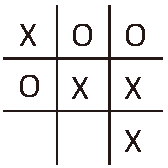
\includegraphics[width=4cm]{c1/img/tic-tac-toc.pdf}
\end{wrapfigure}
回想一下我们所熟悉的儿童游戏——井字棋<tic-tac-toc>. 两个玩家轮流在$3\times 3$的棋盘上下棋. 两个玩家轮流下\textsf{X}与\textsf{O}, 直到一个玩家在水平方向上、垂直方向上或对角线方向上放置了一排的三枚棋子以赢得游戏, 如图中X所做的那样. 如果棋盘填满了而没有任何一名玩家放置出一排三枚棋子, 那么该局比赛就是平局. 因为一名有经验的玩家永远不会输, 让我们假设我们在和一名下棋技术不完美的玩家对战, 他有时会下错来让我们赢得比赛. 让我们暂时假设平局和输掉比赛一样糟糕. 我们该怎样构建一个能发现对手的缺陷并最大化获胜概率的下棋程序呢?

虽然这是一个简单的问题, 但不能使用原有的技术来便利地、令人满意地解决. 例如, 博弈论中的典型的``极小化极大''<minimax>方法在这里是不适用的, 因为其假设了对手下棋的方式. 例如, 一个极小化极大程序永远不会到达一个可能会将其引向失败的状态, 即使在多数情况下因为对手的失误该状态会将其引向胜利. 典型的针对一系列决策问题的优化方法, 例如动态规划<dynamic programming>, 可以\emph{计算}出针对任一对手的方案, 但需要关于对手的完整说明——包括在棋盘的每一个状态中对手下任意一步棋的概率——作为输入. 让我们假设如同实际关注中的多数问题, 这些信息并非先验的. 另一方面, 通过和同一个对手下多盘棋, 这样的信息可以从经验中被评估出来. 对经典方法而言, 关于此问题能做到的最好的就是先学习得到有一定置信度的对手行为模型,  然后对给定的对手近似模型应用动态规划来计算最优解. 最后的这种方法, 和我们之后在本书中探讨的一些强化学习方法没有太大差别.

如果在本问题上应用进化方法, 那么其将在直接在策略空间中搜索可以以高概率战胜对手的策略. 其中, 一个策略即为指导玩家在每一个游戏状态——每一个在$3 \times 3$的棋盘上合法的\textsf{X}与\textsf{O}的配置——中该怎么走的规则. 对于每一个所考虑的策略, 其获胜概率的估计值可以通过与对手下多盘棋来获得. 这样的估计将用于指导哪些策略能够之后继续被考虑. 一个典型的进化算法能在策略空间中逐步提升<hill-climb>, 不停产生并估计策略以获得增量式的改进. 此外, 维持并估计多个策略的遗传算法也可以被使用. 事实上数以百计的优化算法都可以被使用.

接来下讨论井字棋问题怎么利用值函数来处理. 首先我们为每一个可能的状态建立一张数值表. 表中每一个数值都是从该状态起获胜的概率的最新估计值. 我们将此作为每一个状态的\emph{值}<value>, 同时整张表就是学得的值函数. 如果当前, 从状态\textsf{A}起获胜概率的估计值比状态\textsf{B}高, 那么状态\textsf{A}的值比状态\textsf{B}高, 或者说状态\textsf{A}比状态\textsf{B}更``好''. 假设我们一直执\textsf{X}, 那么对所有有一排三枚\textsf{X}棋子的状态其获胜概率为1, 因为在这样的情况下我们已经赢了. 类似的, 对于所有有一排三枚\textsf{O}棋子的状态或平局, 其获胜概率为0, 因为我们已经不可能赢了. 我们将所有其他状态的初始值设为0.5, 表示我们猜测从这些状态起有50\%的概率获胜.

然后我们同对手玩许多盘棋. 为了选择下一步棋, 我们检查下了一步棋之后所有可能的状态(将当前棋盘上任一空填上后各对应一个状态), 然后在表中查找各个状态当前的估计值. 在多数情况下我们\emph{贪心}<greedy>地选择下一步棋, 选择能导向拥有最高值的状态的那步棋, 即选择胜率估计值最高那步棋. 然而, 我们偶尔随机地选择下一步棋. 这些棋被称为\emph{探索}<exploratory>步, 因为这让我们探索原先根本无法经历的状态. 游戏中一系列所考虑与所做出的下法, 被绘制在了\figref{1.1}中.

\begin{figure}[ht]
\begin{center}
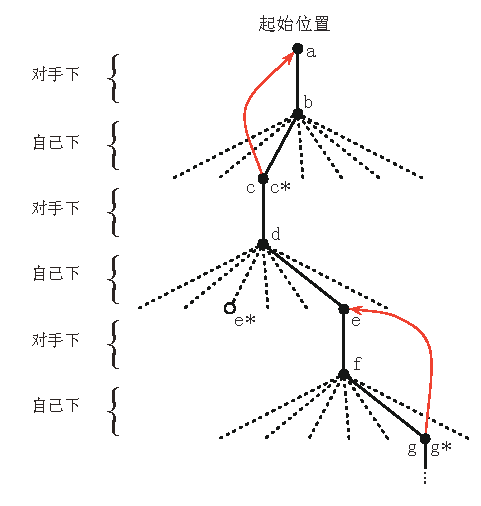
\includegraphics[width=0.7\textwidth]{c1/img/figure1-1.pdf}
\end{center}
\caption{一系列的井字棋下法. 实线表示游戏中实际所下; 虚线表示我们(我们的强化学习程序)考虑了, 但没有实际采用的下法. 我们下的第二步棋是一个探索步, 这意味着另一个同胞节点, 即那个$\mathrm e^*$对应的结点, 估计值更高. 探索步并不能造成学习; 但所有其他的步数可以, 这形成了如图中红色箭头所示的更新, 其中估计值从树的子孙结点流向祖先结点, 细节在正文中叙述.}\label{fig:1.1}
\end{figure}

当我们在下棋时, 我们更改我们经历过的状态的值. 我们尝试做出对获胜率更为准确的估计. 为了做到这一点, 我们将做出贪心选择后的状态值\emph{逆流}<back up>至做出贪心选择前的状态, 如\figref{1.1}所示. 更确切地说, 早先状态的当前值更新后向后续状态的值靠拢. 这可以通过将早先状态的值向后续状态接近部分做到. 让我们用$S_t$表示做出贪心选择前的状态, 用$S_{t + 1}$表示贪心选择后的状态, 那么对$S_t$的值的估计——记作$V(S_t)$——的更新可以写作:
\begin{equation*}
V(S_t) \leftarrow V(S_t) + \alpha[V(S_{t + 1}) - V(S_t)]​,
\end{equation*}
其中$\alpha$为称为\emph{步长}<step-size>的参数, 为一个小的正数, 能影响学习的速率. 上述的更新是\emph{时序差分}<temporal difference, TD>学习方法的特例, 时序差分名称的由来为——更新是基于$V(S_{t + 1}) - V(S_t)$这一两个连续状态的估计值之差.

上述的方法在这个问题上表现很好. 例如, 如果步长参数能随时间以合适的速率递减, 那么对于任何给定的对手, 任意状态的估计值都能收敛到从该状态起我方使用最优策略的话最终获胜的概率. 更进一步说, 收敛后所下的每一步(除去探索步)事实上都是针对这一(非完美)对手的最优下法. 换句话说, 此方法最终收敛为针对这一对手的最优策略. 如果步长参数没有随时间减小到0, 那么下棋程序也能很好地应对缓慢地改变策略的玩家.

这一例子阐明了进化方法与使用值函数的方法的区别. 为了评估一个策略, 进化方法使该策略固定, 同对手下许多盘棋或使用对手的模型模拟下许多盘棋. 获胜的频率给出了该策略获胜概率的无偏估计, 该频率可以用于指导下一步的策略选择. 但策略改进必须要经过许多盘游戏, 并且只有每局游戏的最终结果被利用了——发生在游戏\emph{过程中}的一切都被忽视了. 例如, 如果程序获胜了, 那么这局游戏中的\emph{所有}行为都获得了赞誉<credit>, 无论某一步对获胜而言有多重要. 赞誉甚至被给予从未下过的那几步. 而使用值函数的方法, 与之相反, 允许对各个状态分开进行评估. 从结果上而言, 进化方法与值函数方法都搜索了策略空间, 但对值函数的学习利用了游戏过程中的信息.

这个简单的例子阐明了强化学习方法的一些关键特征. 首先, 在有对手的情况下, 必须强调从与环境的交互中学习. 其次, 必须要有明确的目标, 且正确的动作选择需要将延迟的效果考虑在内的计划或远见. 例如, 简单的强化学习程序可能会学会由多步组成的陷阱, 来应对短视的对手. 这是强化学习方法的一个显著特征: 其不需要对手的模型, 也不需要对未来可能的动作、状态序列进行显式搜索, 就可以达到计划与预见的目的.

虽然这个示例阐明了一些强化学习的基本特征, 但它是在是太简单了, 以致于可能会给人留下强化学习的应用十分有限的印象. 除了井字棋这样的双人游戏外, 强化学习也可以用于没有形式上的对手的情形, 即``与自然斗争的游戏''. 虽然井字棋游戏中每一局是分开的且只在每一局的末尾有奖赏, 但强化学习并不局限于将交互划分为不同分节<episode>的问题. 强化学习也可以应用于交互是无穷无尽的情形, 或可以在任意时间接受不同量级的奖赏的情形. 强化学习甚至可以应用于不像井字棋那样将时间分为离散的步长的问题. 强化学习的一般准则也适用于连续时间<continuous-time>问题, 但相关理论同时也变得更复杂, 因此在此导论性质的书中略去.

虽然井字棋问题的状态集有限且元素数目较小, 但即使状态集很大乃至无限, 强化学习方法也依然适用. 例如, \citet{Tesauro1992, Tesauro1995}将上述算法同人工神经网络结合起来, 并用于有大约${10}^{20}$个状态的西洋双陆棋<backgammon>游戏. 对于这么多状态而言, 即使只经历其中的一小部分也是不可能的. Tesauro的程序的表现远比之前的任何程序好, 并最终超过了顶级人类玩家(\secref{16.1}). 人工神经网络为程序提供了对过去经验进行泛化的能力, 所以当面临新状态时, 程序能通过人工神经网络, 来根据过去面临的类似状态选择合适的下法. 在面临拥有如此庞大的状态集的问题时, 强化学习系统的性能同其能在多大程度上对过去的经验进行泛化密切相关. 在这个主题上, 强化学习最需要监督学习的方法. 为了做到这一点, 人工神经网络与深度学习(\secref{9.6})既不是唯一的方法, 也不一定是最好的方法.

井字棋游戏中, 在学习开始时没有除游戏规则外的任何先验知识, 但强化学习并不一定要从空白开始. 恰恰相反, 先验知识可以以多种方式集成到强化学习中, 且有时这对高效的学习而言是必需的(例如, 参见\secref{9.5}、\secref{17.4}及\secref{13.1}). 此外, 在井字棋游戏中我们可以获取到真实的状态信息, 但强化学习也可以应用于部分状态被隐藏的情形, 或者对学习器而言不同的状态看上去相同的情形.

最后, 井字棋程序能够预见未来, 并预测其所有可能的下法所引出的状态. 但是为了做到这一点, 强化学习程序需要游戏的一个模型, 该模型能预测环境对程序尚未走的那一步的可能反应. 许多问题都类似这样, 但在有些问题中甚至关于短期的动作效果的模型也无法得到. 强化学习在两种情况下都可以适用. 模型并不是必须的, 但如果有现成的模型或模型可以学得, 那么这些模型可以轻而易举地被使用(\chapref{8}).

在另一方面, 存在着不需要任何环境模型的强化学习方法. 免模型系统甚至无法预测环境对单个动作的反应. 使用TD方法的井字棋程序从对手的意义上说是免模型的: 其没有任何种类的关于对手的模型. 因为模型必须要足够准确才能派得上用场, 所以当解决问题的瓶颈在于难以构建足够准确的环境模型时, 免模型方法比其他更复杂的方法有优势. 免模型方法也是有模型方法的重要组件. 本书中, 我们先用数章讨论免模型方法, 然后再讨论其怎样作为更为复杂的有模型方法的组件.

强化学习方法既可以用于系统中的高层, 也可以用于系统中的底层. 虽然在井字棋程序仅学会了游戏的下法, 但没有什么能阻碍将强化学习用于更高的层次中, 其中可能每一个``动作''本身就是复杂的应用. 在层次化学习系统中, 强化学习可以同时工作于多个层级.

\begin{exer}[左右互搏]
假设如果强化学习算法并非与随机的对手对战, 而是自身左右互搏并且两边都进行学习. 你认为这种情况下会发生什么? 其能够学得不同的策略吗?
\end{exer}

\begin{exer}[对称性]
许多井字棋的走法看上去不一样, 但因为对称性的关系本质上是相同的. 我们该怎样修改上述的学习过程来利用这一点? 这一改变会以怎样的形式改善学习过程? 现在, 再思考另一个问题. 假设对手没有利用对称性. 那么在这种情况下, 我们应该利用对称性吗? 对称的位置一定有相等的值吗?
\end{exer}

\begin{exer}[贪心的下法]
假设强化学习程序是贪心的, 即其永远选择能带来最高值的下法. 那么其学得的策略会比非贪心程序更好还是更差? 什么样的问题可能会出现?
\end{exer}

\begin{exer}[从探索中学习]
假设在所有游戏中的所有步之后都进行更新, 包括探索步. 如果步长参数随时间流逝逐渐适当地减小(但探索的可能性不会), 那么各个状态的值会收敛至一个不同的胜率的集合. 从概念上说, 当从或者不从探索步中学习时, 这两个胜率的集合各自是什么? 假设我们继续做出探索步, 那么哪一个胜率的集合可能会更好? 哪一个可能会赢得更多?
\end{exer}

\begin{exer}[其他改进]
你可以想到其他改善强化学习程序的方式吗? 你可以想到更好的用于解决上述的井字棋问题的方法吗?
\end{exer}

\section{总结}\label{sec:1.6}

强化学习是理解并自动化目标导向的学习与决策的计算性方法. 与别的计算性方法的不同之处在于: 其强调从代理与环境的直接交互中学习, 而不需要示范性的训练集或环境的完整模型. 我们认为, 强化学习是第一个真正处理``从与环境的交互中学习来达成长期的目标''这一问题的学科. 

强化学习使用马尔科夫决策过程这一框架, 依据状态、动作与奖赏来定义学习代理与环境之间的交互. 这一框架试图以一种简单的方式表示人工智能问题中的关键特征. 这些特征包括对因果的理解, 对不确定性与概率性的理解, 以及存在有明确的目标.

值与值函数的概念是本书中介绍的多数强化学习方法的关键. 我们认为值函数对于在策略空间中的高效搜索而言是至关重要的. 值函数的使用将强化学习方法同进化方法区别开来, 其中后者通过对整个策略的评估来在策略空间中进行直接搜索.

\section{强化学习的早期历史}\label{sec:1.7}

暂不译

\section*{参考文献}

暂无


\part{表格式方法}\label{part:1}
在本书的这一部分, 我们在强化学习最简单的形式下——状态与动作空间足够小使得近似的值函数可以以数组或\emph{表}<table>来表示——阐述几乎所有强化学习算法的核心概念. 在这种情况下, 这些方法常常可以获得确切的解, 即可以获得确切的最优值函数与最优策略. 这和本书的下一部分叙述的近似方法恰恰相反, 后者只能获得近似解, 但作为回报可以高效地应用于规模大得多的问题上.

本书这一部分的第一章阐述了只有单个状态的强化学习问题特例, 即所谓的赌博机问题. 第二章阐述了在本书的余下部分使用的、一般强化学习问题的形式化——有限马尔科夫决策过程<finite Markov decision process, finite MDP>, 也阐述了形式化中包括了贝尔曼方程<Bellman equation>与值函数的主要概念.

接下来的三章阐述了三类解决有限马尔科夫决策过程的基本方法: 动态规划<dynamic programming, DP>, 蒙特卡洛<Monte Carlo, MC>方法, 以及时序差分<temporal difference, TD>方法. 每一类方法都有其优点与缺点. 动态规划方法在数学上被研究得很好, 但需要完整、正确的环境模型. 蒙特卡洛方法不需要模型且从概念上说较为简单, 但不适合于逐步的增量计算. 最后, 时序差分方法不需要模型且完全是增量式的, 但分析起来更为复杂. 这些方法在效率与收敛速度这些方面也存在着差异.

余下的两章阐述了怎么将这三类方法结合起来以利用各自的优点. 在其中一章我们阐述怎样通过多步自举方法<multi-step bootstrapping method>来将蒙特卡洛方法与时序差分方法的长处结合起来. 在本部分的最后一章, 我们将展示怎样将时序差分学习方法, 与模型学习以及计划方法(例如动态规划)结合起来, 作为完整、统一的表格式强化学习问题的解决方案.

\chapter{多摇臂赌博机}\label{chap:2}

将强化学习同其他类型的学习区分开来的最重要的特征就是: 强化学习使用训练信息来\emph{评估}所采取的动作, 而非使用正确的动作来\emph{指导}动作的选择. 正是这一点提出了对积极探索的要求. 单纯的评估性反馈只能说明所采取的动作的好坏, 但无法说明其是否为最好或最坏的动作. 单纯的指示性反馈, 恰恰相反, 指示出应该做的正确动作, 且独立于实际采取的动作. 这一类的反馈是包含了大量模式分类、人工神经网络、系统辨别的监督学习的基础. 在各自最典型的情况下, 这两类反馈是大不相同的: 评估性反馈完全依赖于所采取的动作, 而指示性反馈独立于所采取的动作.

在本章中我们在简化的设定下——仅需要在单个状态下学得如何采取动作——来探讨强化学习评估的方面. 多数涉及到评估性反馈的先前工作正是在这个\emph{非关联性}<nonassociative>设定下完成的, 因为这个设定避免了完整强化学习问题的复杂性. 学习这种情形使我们能清晰地看到评估性反馈怎样地区别于指示性反馈, 又怎样地可以同指示性反馈结合起来.

我们探讨的非关联性的评估性反馈问题正是$k$-摇臂赌博机问题<$k$-armed bandit problem>的一种简单形式. 我们利用这个问题来介绍一些基本的强化学习方法, 并在之后的章节中拓展这些方法以应用于完整的强化学习问题上. 在本章的末尾, 我们探讨赌博机问题变成关联性——即需要在多个状态下采取动作——时会发生什么, 来向完整的强化学习问题更进一步.

% ----------------------------------- sec2.1 ---------------------------------------------
\section{\texorpdfstring{$k$-摇臂赌博机问题}{k-摇臂赌博机问题}}\label{sec:2.1}

考虑如下的学习问题. 你需要重复地对$k$个不同的选项或动作做出选择. 在每一次选择后你会获得一个实数型的奖赏, 该奖赏是从固定的概率分布中采样获得的, 且该概率分布取决于你所选择的动作. 你的目标在一定的时期内, 如1000个动作选择或\emph{时步}<time step>内, 最大化期望的奖赏和.

这是$k$\emph{-摇臂赌博机问题}<$k$-armed bandit problem>的典型形式, 之所以这么称呼是将其类比于老虎机或``单摇臂赌博机'', 只不过其有$k$个摇臂, 而非1个. 每一次动作选择就像拉下赌博机的摇臂之一, 而奖赏就是中了头奖之后的回报. 在反复的动作选择过程中, 你必须将动作集中到最好的摇臂上来最大化累积奖赏. 另一个类比为, 医生为一批批的重病患者选择实验性的疗法. 每一个动作就是选择一种疗法, 而每一个奖赏就是病人存活或健康与否. 现如今术语``赌博机问题''有时也用于上述问题的泛化, 但本书中我们仅用其指代如上所述的简单形式.

在我们的$k$-摇臂赌博机问题中, $k$个动作中的每一个动作都各自有其期望或平均的奖赏; 让我们将其称为该动作的\emph{值}<value>. 我们将在时步$t$选择的动作记为$A_t$, 对应的奖赏记为$R_t$. 任一动作$a$的值, 记为$q_*(a)$, 为$a$被选择后的期望奖赏:
\begin{equation*}
q_*(a) \doteq \mathbb E [R_t \mid A_t = a].
\end{equation*}
如果你知道了每个动作的值, 那么解决$k$-摇臂赌博机问题就很简单了: 只要一直选择值最高的动作即可. 我们假设你不能确定动作值, 虽然你可能有其估计值. 我们将动作$a$在时步$t$的估计值记为$Q_t(a)$. 我们希望$Q_t(a)$尽可能接近$q_*(a)$.

如果你维持有对动作值的估计, 那么在任何时步一定至少有一个动作有着最高的估计值. 我们将其称为\emph{贪心}<greedy>动作. 当你选择贪心动作之一时, 我们称你在\emph{利用}<exploit>你对动作值的已有知识. 但如果你选择了非贪心动作之一, 那么我们称你在\emph{探索}<explore>, 因为这能帮助你改进对非贪心动作的值的估计. 利用用于最大化单步的期望奖赏, 但探索也许可以在长期内产生更高的奖赏和. 例如, 假设一个贪心动作的值是确定地知道的, 而一些其他的动作以极高的不确定性被估计为和贪心动作差不多好. 这个不确定性为, 这些动作中的至少一个动作, 可能比贪心动作要好, 但你不知道是哪一个. 如果你在选择动作前有许多时步的话, 那么这么做也许会更好: 探索非贪心动作, 来发现其中哪个比贪心动作更好. 在探索过程中, 短期而言奖赏变低了, 但长期而言奖赏会变高, 因为在你发现了更好的动作后, 你可以穿多次地利用\emph{它们}. 因为在单个动作选择中不能既探索又利用, 所有这常常被称为探索与利用之间的``矛盾''.

在任何一个具体的情况下, 是探索还是利用更好取决于对估计值、不确定性、余下步数的具体值的复杂考量. 有许多针对$k$-摇臂赌博机及其关联问题的特定数学形式的、用于平衡探索和利用的精巧方法. 然而, 这些方法中的多数对固定性<stationarity>及先验知识做出了较强的假设, 这些假设对实际应用或我们在接下来的章节中考虑的完整的强化学习问题而言, 要么无法做到, 要么无法证实. 就这些方法而言, 当这些假设不成立时, 其对最优性的保证或对损失的边界的保证, 都无从谈起. 

在本书中我们不考虑以精妙的方式平衡探索和利用; 我们仅以浅显的程度对平衡方法进行探讨. 在本章中我们将呈现数种针对$k$-摇臂赌博机问题的平衡方法, 以及其对只会利用的方法的显著优越性. 需要平衡探索和利用是强化学习特有的特有的挑战; 我们这一版本的$k$-摇臂赌博机问题的简洁性, 使我们能够以一种特别清晰的形式来呈现这一点.

% ----------------------------------- sec2.2 ---------------------------------------------
\section{动作值方法}\label{sec:2.2}

我们以对两种方法的更进一步的审视开始. 这两种方法分别为估计动作值的方法, 以及使用估计值来做出动作选择的决策的方法, 两者合称为\emph{动作值方法}<action-value method>. 我们还记得一个动作的真实值是该动作被选择时的平均奖赏. 一个自然的估计方法就是对接受到的奖赏进行平均:
\begin{equation}\label{eq:2.1}
Q_t(a) = \frac{\text{时步$t$之前采取动作$a$所获得奖赏之和}}{\text{时步$t$之前采取动作$a$的次数}} = \frac{\sum_{i=1}^{t-1}{R_i} \cdot \mathbbm{1}_{A_i = a}}{\sum_{i=1}^{t-1}{\mathbbm{1}_{A_i = a}}}, 
\end{equation}
其中$\mathbbm{1}_{predicate}$表示一随机变量, 当谓词predicate为真时其值为1, 反之为0. 如果分母为0的话, 那么我们可以将$Q_t(a)$设定为一默认值, 比如0. 当分母趋向于无穷大时, 由大数定理可以得知$Q_t(a)$收敛于$q_*(a)$. 我们将此称为估计动作值的\emph{样本平均}方法<sample-average method>, 因为估计值为相关奖赏的样本的均值. 当然这只是估计动作值的一种方法, 也不一定是最好的一种. 但是, 让我们暂且使用这种简单的估计方法, 然后考虑怎样使用估计值来选择动作的问题.

最简单的动作选择规则就是选择有最高估计值的那个动作, 即前一节中定义的贪心动作. 如果有多于一个的贪心动作, 那么以任意一种方式在选择其中一个, 例如随机选择. 我们将这样的\emph{贪心}<greedy>动作选择写作
\begin{equation}\label{eq:2.2}
A_t = \dargmax Q_t(a),
\end{equation}
其中$\targmax_a$表示令后面的表达式最大的那个动作$a$(再次声明, 如果有多个最值时任意选择). 贪心选择总是对已有的知识进行利用来最大化立即的奖赏; 其不会对明显次等的动作进行采样来观察这些动作是否实际上更好. 一个简单的替代方法就是在多数的时间内进行贪心选择; 但是每隔一定时间, 如以一个较小的概率$\varepsilon$, 从所有的动作中以相同的概率进行随机选择, 无论各个动作的估计值为多少. 我们将使用这种近似贪心的动作选择规则的方法称为$\varepsilon$-贪心方法. 这一方法的优点是, 当步数增加到无穷大时, 每个动作都会被采样无穷多次, 因此保证了所有的$Q_t(a)$都收敛到$q_*(a)$. 这也预示着选择最优动作的概率会收敛到大于$1 - \varepsilon$的值, 即几乎确定. 然而这只是一个渐进的保证, 且无法说明该方法的实际效率. 

\begin{exer}
对于$\varepsilon$-贪心动作选择, 在有两个动作并且$\varepsilon = 0.5$的情况下, 贪心动作被选择的概率是多少.
\end{exer}

% ----------------------------------- sec2.3 ---------------------------------------------
\section{10-摇臂测试工具}\label{sec:2.3}

为了大致地评估贪心与$\varepsilon​$-贪心动作值方法的相对效率, 我们使用一个测试问题套件来定量地比较它们. 这是一个由2000个随机生成的$k​$-摇臂赌博机问题组成的集合, 其中$k = 10​$. 对每个赌博机问题而言, 如在\figref{2.1}中所展示的, 各个动作值$q_*(a), \; a= 1, \dots, 10​$, 是从均值为0且方差为1的正态(高斯)分布中采样得到的. 并且, 若一个应用于本问题的学习方法在时步$t​$时选择了动作$A_t​$, 那么实际奖赏$R_t​$是从均值为$q_*(A_t)​$且方差为1的正态分布中采样获得的. 这些分布在\figref{2.1}中用灰色表示. 我们将这个测试任务套件称为\emph{10-摇臂测试工具}. 对于任何学习方法来说, 当将其应用于赌博机问题之一时, 我们可以测量其于1000多个时步中逐步提升的性能与表现. 这构成了一个\emph{行程}<run>. 将此重复2000个独立的行程, 且每个行程使用不同的赌博机问题, 我们获得了对学习算法的平均表现的度量.

\begin{figure}[ht]
\centering
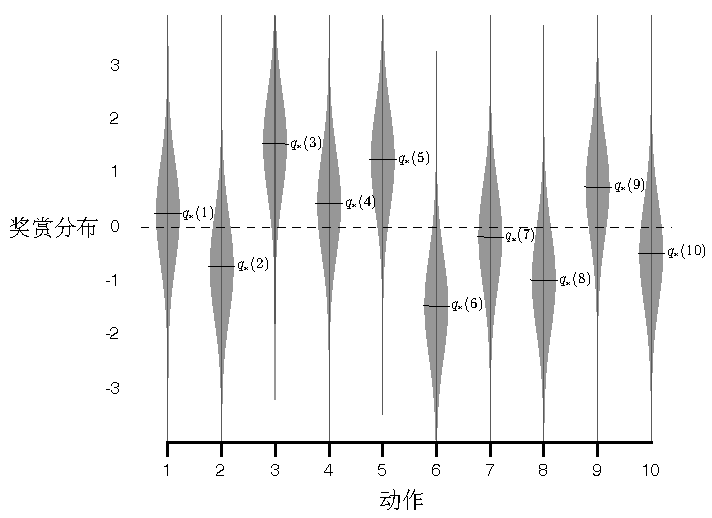
\includegraphics[width=.8\textwidth]{c2/img/figure2-1.pdf}
\caption{一个来自10-摇臂测试工具的赌博机问题示例. 10个动作的真实值$q_*(a)$是从均值为0且方差为1的正态分布中采样得到的, 并且实际奖赏是从均值为$q_*(a)$且方差为1的正态分布中采样得到的.}\label{fig:2.1}
\end{figure}

使用如上所述的10-摇臂测试工具, 对贪心方法以及两个$\varepsilon$-贪心方法($\varepsilon = 0.01$及$\varepsilon = 0.1$)进行对比, 结果如\figref{2.2}所示. 所有方法都使用采样平均方法来估计动作值. 上侧的图展示了随经历增长的期望奖赏. 在最开始, 贪心方法比其他两个方法增长得稍微快一点, 但在一个很低的水平就趋于平稳了. 其只达到了单步奖赏约为1的水准, 而在此测试工具上单步奖赏可能的最大值约为1.55. 贪心方法在长期过程中表现明显相对其他方法更差, 因为其常常陷于对次优动作的选择中. 下侧的图显示贪心方法在大约三分之一的任务中找到了最优动作. 在余下的三分之二任务中, 其对最优动作的初始采样值偏低, 因此最优动作从未被再次选择. $\varepsilon$-贪心方法最终表现得比贪心方法更好, 因为前者持续探索并持续提高发现最优动作的可能. $\varepsilon = 0.1$的方法探索得更多, 所以常常更早地发现最优动作, 但其从不会以超过91\%的概率选择该动作. $\varepsilon = 0.01$的方法提升得更为缓慢, 但最终会在图中的两种测度上比$\varepsilon = 0.1$的方法表现得更好. 也可以随时间逐步减小$\varepsilon$来吸收高$\varepsilon$与低$\varepsilon$值的优点.

\begin{figure}[ht]
\centering
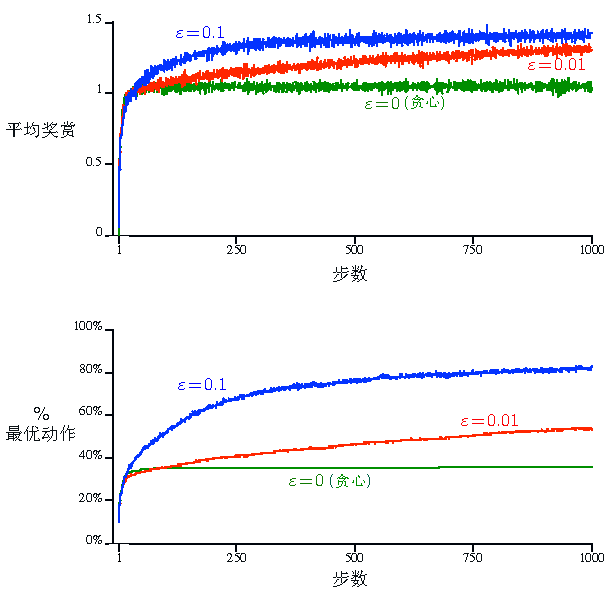
\includegraphics[width=.7\textwidth]{c2/img/figure2-2.pdf}
\caption{$\varepsilon$-贪心动作值方法在10-摇臂测试工具上的平均表现. 这些数据是对超过2000次使用不同赌博机问题的行程中的数值的平均. 所有的方法使用采样平均方法估计动作值.}\label{fig:2.2}
\end{figure}

$\varepsilon$-贪心方法对贪心方法的优势视任务而定. 例如, 假设奖赏的方差变得更大, 比如是10而不是1. 对于有更多噪声的奖赏, 代理需要更多的探索来发现最优动作, 那么$\varepsilon$-贪心方法的优势甚至会更大. 在另一方面, 如果奖赏的方差为0, 那么贪心方法在试过一次后就可以得知所有动作的真实值. 在这种情况下贪心方法可能是表现得最好的, 因为其立即发现了最优解, 然后不再做任何探索. 但如果我们弱化一些假设, 即使是在确定性<deterministic>\footnote{表示概率为1, 如上述的方差为0的情形, 与下述的(非)固定性在意义上不同}情况下, 探索也能很有优势. 例如, 假设赌博机问题是非固定性<nonstationary>的, 即动作的真实值会随时间变化. 在这种情况下, 即使有确定性这一性质的存在, 依然需要探索来保证没有一个非贪心动作变得比贪心动作更好. 就像我们在接下来的几章看到的那样, 非固定性情况在强化学习中最为常见. 即使潜在的任务是确定性与固定性的, 学习器也可能面临一组这样的任务, 其中每个任务都随着学习的进行和代理的决策策略的变化而随时间改变. 强化学习需要对探索与利用的平衡.

\begin{exer}[赌博机例子]
考虑一个$k = 4$的$k$-摇臂赌博机问题, 其中各个摇臂分别记为1, 2, 3, 4. 将一赌博机算法应用于该问题, 该算法使用$\varepsilon$-贪心动作选择与样本平均动作值估计方式, 且对所有的动作$a$, 初始估计值$Q_1(a) = 0$. 假设最开始的动作与奖赏序列为$A_1 = 1$, $R_1 = -1$, $A_2 = 2$, $R_2 = 1$, $A_3 = 2$, $R_3 = -2$, $A_4 = 2$, $R_4 = 2$, $A_5 = 3$, $R_5 = 0$. 其中有些时步$\varepsilon$情况发生了, 使得一个动作被随机选择. 在哪些时步中这一定发生了? 在哪些时步中可能发生了?
\end{exer}

\begin{exer}
在\figref{2.2}的比对中, 从长期来看, 哪种方法会在累积奖赏和选择最优动作的概率方面表现最佳? 该方法会比其他方法好多少? 请定量地表达你的观点.
\end{exer}

% ----------------------------------- sec2.4 ---------------------------------------------
\section{增量式实现}\label{sec:2.4}

我们至今讨论的动作值方法全都使用观察到的奖赏的样本均值来估计动作值. 我们现在转向``这些平均值应该怎样才能以高效的方式被计算出来''这一问题, 更具体地说, 怎样以常数的内存使用与每一时步中常数的计算时间计算出来. 

为了简化标记, 我们将专注于单个动作上. 让$R_i$表示在第$i$次选择该动作后接收到的奖赏, 并以$Q_n$表示在选择了$n - 1$次该动作后其估计值, 现在我们可以简单地将$Q_n$写作
\begin{equation*}
Q_n \doteq \frac{R_1 + R_2 + \dots + R_{n - 1}}{n - 1}.
\end{equation*}
最显而易见的实现方式就是维持对所有接收到的奖赏的记录, 然后每当需要估计值的时候就计算上方的等式. 然而, 以这种方式实现的话, 对内存与计算时间的需求会随着越来越多的奖赏被观察到而逐步增大. 每一个新观察到的奖赏都会需要额外的内存来存储, 需要额外的计算时间来计算分子中的和.

就像你怀疑的那样, 这事实上并不是必需的. 很简单就能发明增量式地更新均值的公式, 且只需要极小的、常数的计算时间来处理每个新奖赏. 给定$Q_n$和第$n$次的奖赏$R_n$, 所有$n$个奖赏的新的均值可以使用下式计算
\begin{equation}\label{eq:2.3}
\begin{aligned}[b]
Q_{n + 1} &= \frac{1}{n} \sum_{i = 1}^n R_i \\
&= \frac{1}{n} \left( R_n + \sum_{i = 1}^{n - 1}R_i \right) \\
&= \frac{1}{n} \left( R_n + (n - 1) \frac{1}{n - 1} \sum_{i = 1}^{n - 1}R_i \right) \\
&= \frac{1}{n} \left( R_n + (n - 1) Q_n \right) \\
&= \frac{1}{n} \left( R_n +n Q_n - Q_n \right) \\
&= Q_n + \frac{1}{n} \left[ R_n - Q_n \right],
\end{aligned}
\end{equation}
上述的等式甚至在$n = 1$时也成立, 即$Q_2 = R_1$, 对任意$Q_1$均成立. 这一实现方式只需要存储$Q_n$和$n$的内存, 以及对每个新奖赏使用\eqref{eq:2.3}的极小的计算时间.

更新规则\eqref{eq:2.3}属于一种在全书中经常出现的更新形式. 这一一般形式为
\begin{equation}\label{eq:2.4}
\begin{aligned}[b]
\text{新估计值} &\leftarrow \text{旧估计值} + \text{步长} [\text{目标} - \text{旧估计值}] \\
(NewEstimate &\leftarrow OldEstimate + StepSize [Target - OldEstimate])
\end{aligned}
\end{equation}
表达式$[\text{目标} - \text{旧估计值}]$是估计中的\emph{误差}<error>. 通过向``目标''靠近来减小该误差. 假定上, 目标预示着希望的移动方向, 虽然这可能是有噪声的. 例如在前述的情形中, 目标就是第$n$次奖赏.

\begin{pcbox}{一个简单的赌博机算法}{!ht}
\pcind[0] 初始化, for $a = 1$ to $k$: \\
\pcind[1] $Q(a) \leftarrow 0$ \\
\pcind[1] $N(a) \leftarrow 0$ \\
\pcind[0] Loop forever:\\
\pcind[1] $A \leftarrow \begin{cases} \targmax_a Q(a) &\text{以}1-\varepsilon\text{的概率(若多个最值, 随意选择)}\\ \text{一个随机动作} & \text{以}\varepsilon \text{的概率} \end{cases}$ \\
\pcind[1] $R \leftarrow bandit(A)$ \\
\pcind[1] $N(A) \leftarrow N(A) + 1$ \\
\pcind[1] $Q(A) \leftarrow Q(A) + \frac{1}{N(A)}[R - Q(A)]$
\end{pcbox}

注意在增量式方法\eqref{eq:2.3}中步长参数会随时间变化. 在处理对动作$a$的第$n$次奖赏时, 该方法使用的步长参数为$\frac{1}{n}$. 在本书中我们将步长参数记为$\alpha$, 或更为一般的, 记为$\alpha_t(a)$.

% ref warning
使用增量式计算的样本均值与$\varepsilon$-贪心动作选择的完整赌博机算法的伪代码展示在了前一页的方框内. 函数$bandit(a)$假定为以动作为参数, 返回相应奖赏的函数.


% ----------------------------------- sec2.5 ---------------------------------------------
\section{追踪非固定性问题}\label{sec:2.5}

我们至今讨论的平均方法可以适用于固定性赌博机问题, 即奖赏的概率分布不会随时间变化的赌博机问题. 就像之前指出的那样, 实际上我们经常遇到非固定性的强化学习问题. 在这种情况下, 相对于较早的奖赏, 将更多的权重给予较近的奖赏是很有意义的. 最为流行的、能做到这一点的方法之一就是使用固定的步长参数. 例如, 对过去的$n - 1$次奖赏的平均, $Q_n$, 其增量式更新规则\eqref{eq:2.3}可以改写为
\begin{equation}\label{eq:2.5}
Q_{n + 1} \doteq Q_n + \alpha [R_n - Q_n],
\end{equation}
其中步长参数$\alpha \in (0, 1]$, 为一常数. 这使得了$Q_{n + 1}$成为了对过去奖赏与初始估计值$Q_1$的加权平均:
\begin{equation}\label{eq:2.6}
\begin{aligned}[b]
Q_{n + 1} &= Q_n + \alpha [R_n - Q_n] \\
&= \alpha R_n + (1 - \alpha) Q_n \\
&=  \alpha R_n + (1 - \alpha) [\alpha R_{n - 1} + (1 - \alpha)Q_{n - 1}] \\
&=  \alpha R_n + (1 - \alpha) \alpha R_{n - 1} + (1 - \alpha)^2 Q_{n - 1} \\
&=  \alpha R_n + (1 - \alpha) \alpha R_{n - 1} + (1 - \alpha)^2 \alpha R_{n - 2} + \dots + (1 - \alpha)^{n - 1} \alpha R_1 + (1 - \alpha)^n Q_1 \\
&= (1 - \alpha)^n Q_1 + \sum_{i = 1}^n \alpha (1 - \alpha)^{n - i} R_i.
\end{aligned}
\end{equation}
我们将此称为加权平均, 因为权重之和$(1 - \alpha)^n + \sum_{i = 1}^n \alpha (1 - \alpha)^{n - i} = 1$, 读者可以自行证明. 请注意给予奖赏$R_i$的权重$\alpha (1 - \alpha)^{n - i}$取决于在多少次奖赏前该奖赏被观察到, 即$n - 1$的值. $1 - \alpha$的值小于1, 因此给予$R_i$的权重会随着与迄今间隔的奖赏次数增加而减少. 事实上, 因为以$1 - \alpha$为底的指数因子的存在, 该权重会指数衰减(如果$1 - \alpha = 0$, 那么所有的权重都集中于最新的奖赏$R_n$, 因为依照惯例$0^0 = 1$). 所以, 这有时也被称为\emph{指数新近加权平均}<exponential recency-average>.

有时, 在每一步都改变步长参数可以提供便利. 令$\alpha_n (a)$表示用于处理第$n$次选择动作$a$后所收到奖赏的步长参数. 如我们之前所说, 若$\alpha_n (a) = \frac{1}{n}$, 即为采样平均方法, 而依据大数定理其确保能收敛到真实的动作值. 但理所当然, 不是所有的序列选择${\alpha_n(a)}$都确保能收敛. 一个随机逼近理论<stochastic approximation theory>中的著名结论, 为我们提供了能以1的概率保证收敛的条件:
\begin{equation}\label{eq:2.7}
\sum_{n = 1}^\infty \alpha_n(a) = \infty  \; \text{且} \; \sum_{n = 1}^\infty \alpha_n^2(a) < \infty
\end{equation}
我们需要第一个条件来保证这些步长对``最终克服初始条件或随机波动的影响''而言足够大. 第二个条件确保最终步长变得足够小以确保收敛. 

请注意采样平均的情形, 即$\alpha_n(a) = \frac{1}{n}$, 满足上述两个条件; 而步长恒定的情形, 即$\alpha_n(a) = \alpha$, 并非如此. 对后者而言, 其并不能满足第二个条件, 这意味着估计值不会完全收敛, 而是继续随新收到的奖赏变化. 就像我们之前提到过的那样, 这事实上正是非固定性环境所需要的, 而实际上非固定性问题在强化学习中是最为常见的. 此外, 满足条件\eqref{eq:2.7}步长参数序列常常收敛得非常缓慢或需要大量的调参来获得令人满意的收敛速率. 虽然满足上述收敛条件的步长参数序列常常用于理论研究中, 但极少用于实际应用或实证研究中.

\begin{exer}
如果步长参数$\alpha_n$不是常数, 那么估计值$Q_n$为对之前所收到奖赏的加权平均, 且权重与\eqref{eq:2.6}给出的不同. 那么类比于\eqref{eq:2.6}, 怎么使用步长参数序列, 来表示一般情形下的各个已收到的奖赏的权重?
\end{exer}

\begin{exer}
设计并实现一个实验, 来解释样本平均方法在处理非固定性问题时所面临的困境. 可以使用10-摇臂测试工具的修改版本, 其中所有的$q_*(a)$初始值相同, 然后独立地随机变动(例如在每一步, 向各个$q_*(a)$添加采样自均值为0且标准差为0.01的正态分布的增量). 然后为以下两种动作值方法绘制类似\figref{2.2}的图表: 其一使用增量式计算的样本平均法; 其二使用恒定步长参数$\alpha = 0.1$. 此外, 令$\varepsilon = 0.1$, 并且使用更长的行程, 例如10,~000步.
\end{exer}

% ----------------------------------- sec2.6 ---------------------------------------------
\section{乐观初始值}\label{sec:2.6}

我们至今讨论的所有方法或多或少依赖于初始的动作值的估计值, $Q_1(a)$. 用统计学的术语来说, 这些方法因初始的估计值产生了偏差<bias>. 对于样本平均方法来说, 当所有的动作都被选择了一次后偏差就消失了; 但对$\alpha$值恒定的方法来说, 这一偏差会永远存在, 但会随时间逐步减小, 正如\eqref{eq:2.6}所示. 在实际应用中, 这类偏差常常并不成问题, 反而有时还很有帮助. 其负面影响是初始值实际上变成了一组必须由用户选择的参数, 要是能将它们都设为0的话该多好. 其正面影响是提供了一种简单的方式, 来应用关于预期的奖赏值的水平的先验知识.

初始动作值也可以以一种简单的鼓励探索的方式来使用. 如果我们在10-摇臂测试工具中, 不是将初始动作值都设为0, 而是将其都设为$+5$. 我们还记得在该问题中$q_*(a)$是从均值为0且方差为1的正态分布中采样得到的. 因此$+5$的初始估计值是极为乐观的. 但这份乐观鼓励了动作值方法去探索. 无论开始时选择了哪个动作, 收到的奖赏都低于初始估计值; 学习器因此对收到的奖赏感到``失望'', 转而选择别的动作. 结果就是所有的动作都在估计值收敛前被选择了数次. 即使一直选择贪心动作, 强化学习系统事实上也做了大量的探索.

\figref{2.3}展示了$Q_1(a) = +5$的贪心方法在10-摇臂测试工具上的表现. 作为对比, $Q_1(a) = 0$的$\varepsilon$-贪心方法也展示在了图中. 最开始, 乐观方法表现得比$\varepsilon$-贪心方法差, 但因为乐观方法的探索随时间流逝减少, 因此最终乐观方法的表现好于$\varepsilon$-贪心方法. 我们将这一鼓励探索的技术称为\emph{乐观初始值}<optimistic initial values>. 我们将其视作一个在固定性问题上可以表现得非常高效的小技巧, 但其远不能成为一个通用的有效鼓励探索的方法. 例如, 其不适宜于非固定性问题, 因为其对探索的驱动本质上是暂时的. 如果任务变化并对探索产生了新的需求, 那么这一方法就无能为力了. 事实上, 以任何特定的方式关注于初始值的方法都对一般的非固定性问题无能为力. 时间上的开端只会出现一次, 因此我们不应该对开端过分关注. 这一评判也适用于样本平均方法, 其也将时间上的开端作为特别事件, 并以均等的权重来平均所有的后续奖赏. 话虽如此, 所有这些方法都很简单, 且这些方法中的一个或多个的组合常常对实际应用而言足够了. 在本书的余下部分中我们将频繁使用这些简单的探索技术.

\begin{figure}[ht]
\centering
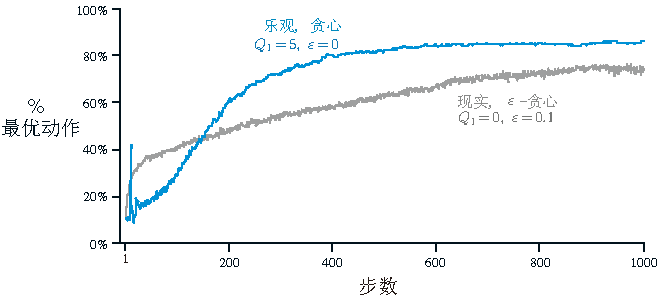
\includegraphics[width=.75\textwidth]{c2/img/figure2-3.pdf}
\caption{乐观的动作值初始估计在10-摇臂测试工具上的表现. 两种方法都使用了恒定步长参数$\alpha = 0.1$.}\label{fig:2.3}
\end{figure}

\begin{exer}[神秘的尖峰]
\figref{2.3}中显示的结果应该是很可靠的, 因为其为2000个独立的、随机选择的10-摇臂赌博机问题上的结果的平均. 那么在乐观方法的曲线的开始部分为什么会有震荡与尖峰? 换句话说, 是什么使得这一方法在特定的较早时步中, 从平均的意义上说表现得特别好或特别差?
\end{exer}

\begin{exer}[无偏的恒定步长技巧]
在本章的多数部分中我们使用了样本均值来估计动作值, 因为样本平均法不会产生如恒定步长方法所拥有的初始偏差(具体见导出\eqref{eq:2.6}的分析). 然而, 样本平均方法可能不是一个完全令人满意的解决方案, 因为其在非固定性问题上表现不佳. 有没有可能避免恒定步长带来的偏差又保持其在非固定性问题上的优势? 一种方法是使用如下步长
\begin{equation}\label{eq:2.8}
\beta_n \doteq \alpha / \bar{o}_n,
\end{equation}
来处理第某一动作带来的第$n$次的奖赏, 其中$\alpha > 0$, 是常规的恒定步长, 而$\bar{o}_n$为从0开始逐步靠近1的序列:
\begin{equation}\label{eq:2.9}
\bar{o}_n = \bar{o}_{n - 1} + \alpha (1 - \bar{o}_{n - 1}), \; \text{对} n \geq 0 \text{, 且其中} \bar{o}_0 \doteq 0
\end{equation}
做出如\eqref{eq:2.6}中的分析来证明$Q_n$是无初始偏差的指数新近衰减平均.
\end{exer}

% ----------------------------------- sec2.7 ---------------------------------------------
\section{上置信界动作选择}\label{sec:2.7}

因为对动作值估计的准确度的不确定性存在, 所以需要进行探索. 贪心动作是当前看上去最好的动作, 但其他动作中的一些可能事实上更好. $\varepsilon$-贪心动作选择强制使得非贪婪动作被选择, 但这一过程对各个动作是不加区分的, 即使是接近贪心或特别不确定的动作也不被偏好. 对非贪心动作来说, 将其估计值离成为最大值的距离与估计值中的不确定性考虑在内, 由此判断各个非贪心动作成为最优动作的潜力, 然后根据这个潜力进行动作动作选择显然是更好的. 一种能做到这一点的高效方式就是由下式进行动作选择
\begin{equation}\label{eq:2.10}
A_t \doteq \underset{a}{\operatorname{argmax}} \left[ Q_t(a) + c \sqrt{\frac{\ln t}{N_t(a)}} \;\right],
\end{equation}
其中$\ln t$表示$t$的自然对数($e \approx 2.71828$的该数次幂等于$t$), $N_t(a)$表示在时间$t$之前动作$a$被选择的次数(\eqref{eq:2.1}中的分母), 以及常数$c > 0$控制了探索的程度. 如果$N_t(a) = 0$, 那么$a$被认为是最优动作.

如上所述的\emph{上置信界}<upper confidence bound, UCB>动作选择的观念为: 式中的根号项是对$a$的估计值的不确定度或方差. 欲寻求最大值的项\footnote{即$\dargmax_a$右侧的量, 译者注}, 是动作$a$可能的真实值的上界的一种, 其中由$c$决定置信水平. 每当$a$被选择时, 不确定性可以被认为是减少了: $N_t(a)$增加, 因为其出现在分母中, 所以不确定性项减小了. 在另一方面, 每当除$a$之外的动作被选择, $t$增加而$N_t(a)$保持不变; 因为$t$出现在分子中, 所以对不确定性的估计增加了. 自然对数的使用意味着增长的速率逐渐变慢, 但其值依然会趋近于无穷大; 所有的动作都会被选择, 但有较低的估计值或已经被频繁选择过的动作, 将会随时间推移减少被选择的频率. 在10-摇臂测试工具上使用UCB的结果如\figref{2.4}所示. 像图中所展示的那样, UCB常常表现得很好, 但相比于$\varepsilon$-贪心而言, 其更难以从赌博机问题拓展到书中余下部分中的, 更为一般的强化学习情形. 其中的一个困难之处就是对非固定性问题的处理——需要比\secref{2.5}中所呈现的更为复杂的方法. 另一个困难之处出现于对巨大状态空间的处理, 特别是当使用了如本书\partref{2}所述的函数近似方法时. 在这些更为复杂的情形下, UCB动作选择通常是不理想的. 

\begin{figure}[ht]
\centering
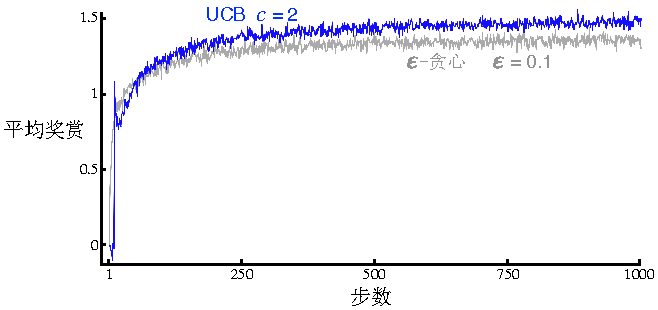
\includegraphics[width=.75\textwidth]{c2/img/figure2-4.pdf}
\caption{UCB动作选择在10-摇臂测试工具中的平均表现. 如图所示, 除了UCB从尚未尝试过的动作中随机进行选择的起始$k$步外, UCB通常表现得比$\varepsilon$-贪心动作选择好.}\label{fig:2.4}
\end{figure}

\begin{exer}[UCB尖峰]
在\figref{2.4}中UCB算法的表现在第11步时有一个明显的尖峰. 为什么会这样? 请注意, 为了使答案完全令人满意, 其需要从``为什么奖赏在第11步增加了?'', 以及``为什么奖赏又在后续的几步中减小了?''这两个方面进行解释. 提示: 如果$c = 1$, 那么尖峰将更矮.
\end{exer}

% ----------------------------------- sec2.8 ---------------------------------------------
\section{梯度赌博机算法}\label{sec:2.8}

在本章的之前部分, 我们已经学习了对动作值进行估计, 然后使用估计值来选择动作的多种方法. 这常常是一种好的途径, 但并不是唯一的途径. 在本节中, 我们将考虑如何为每一个动作$a$学得各自实数型的\emph{偏好}<pautoreference>, 我们将其记为$H_t(a)$. 偏好值越高, 那么对应的动作越常被采用, 但是偏好不能使用奖赏的观念来理解. 只有一个动作相较于另一个动作的相对偏好值是有意义的; 如果我们将所有动作的偏好值加上1000, 各个动作被选择的概率仍然保持不变, 其中概率是由如下的\emph{soft-max分布}(也称为Gibbs分布或Boltzmann分布)决定的:
\begin{equation}\label{eq:2.11}
\Pr\{A_t = a\} \doteq \frac{e^{H_t(a)}}{\sum_{b = 1}^{k} e^{H_t(b)}} \doteq \pi_t(a),
\end{equation}
这里我们引入一种实用的新标记$\pi_t(a)$, 来表示在时步$t$采取动作$a$的可能性. 起始时, 所有动作的偏好值都是相等的(例如对所有的a来说, $H_1(a) = 0$), 因此所有动作都有相同的被选择的概率.

\begin{exer}
证明在只有两个动作的情况下, soft-max分布, 和统计学及人工神经网络中常用的logistic或sigmoid函数给出的分布是等价的.
\end{exer}

基于随机梯度上升<stochastic gradient ascent>, 可以自然地得到这一设定下的学习算法. 在每一步时, 在选择动作$A_t$并收到奖赏$R_t$后, 动作偏好值使用下式进行更新:
\begin{equation}\label{eq:2.12}
\begin{aligned}[b]
H_{t + 1}(A_t) &\doteq H_t(A_t) + \alpha (R_t - \bar{R}_t)(1 - \pi_t(A_t)), &&\text{且} \\
H_{t + 1}(a) &\doteq H_t(a) - \alpha(R_t - \bar{R}_t) \pi_t(a), &&\text{对所有的}a \neq A_t,
\end{aligned}
\end{equation}
其中$\alpha > 0$, 为步长参数, 且$\bar{R}_t \in \mathbb{R}$, 为时步$t$及之前的所有奖赏的平均, 可以如\secref{2.4}(如果问题是非固定性的话, 那么如\secref{2.5})中所述的那样进行增量式的计算. $\bar{R}_t$这一项是作为比较奖赏的基准线的. 如果奖赏高于基准线, 那么将来采取动作$A_t$的概率将增加; 反之如果奖赏低于基准线, 那么概率将减小. 而未被选择的动作的概率朝相反方向移动.

\begin{figure}[!ht]
\centering
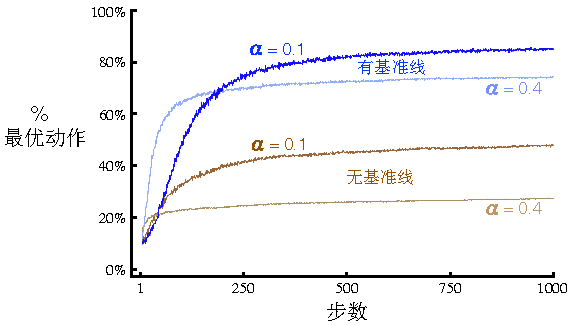
\includegraphics[width=.7\textwidth]{c2/img/figure2-5.pdf}
\caption{在$q_*(a)$接近+4而非0的10-摇臂测试工具上, 有无奖赏基准线的梯度赌博机算法的平均表现.}\label{fig:2.5}
\end{figure}

\figref{2.5}展示了梯度赌博机算法在10-摇臂测试工具的变体上的结果, 该变体中真实的期望奖赏是从一均值为$+4$而非0(方差和从前一样为1)的正态分布中采样获得的. 所有奖赏的同时增加对梯度赌博机算法绝对没有影响, 因为奖赏的基准线会立即适应到新的水平上. 但如果基准线被省略了(即如果\eqref{eq:2.12}中的$\bar{R}_t$恒取0), 那么其性能将如图中所示的那样急剧退化.

\FloatBarrier
\begin{mathbox}{作为随机梯度上升的梯度赌博机算法}
我们可以将梯度赌博机算法理解为梯度上升的概率性近似, 来获得更深入的理解. 在典型的\emph{梯度上升}<gradient ascent>中, 各个动作的偏好值$H_t(a)$将会正比于增量在表现<performance>上的效果而增加:
\begin{equation}\label{eq:2.13}
H_{t + 1}(a) \doteq H_t(a) + \alpha \frac{\partial \mathbb{E}[R_t]}{\partial H_t(a)},
\end{equation}
其中表现上的度量即为奖赏的期望值:
\begin{equation*}
\mathbb{E}[R_t] = \sum_x \pi_t(x) q_*(x),
\end{equation*}
且对增量的效果的度量为: 表现上的度量相对于动作偏好值的\emph{偏导数}. 当然, 因为假设上我们不知道$q_*(x)$, 所以不可能在现有情况下实现典型的梯度上升, 但事实上从期望值的角度看, 算法\eqref{eq:2.12}中的更新等同于\eqref{eq:2.13}中的更新, 这使得前者成为了\emph{随机梯度上升}方法的实例. 证明这一点的推导只需要初等的微积分知识, 但是需要花费数步. 首先让我们更近地看一看表现的梯度:
\begin{equation*}
\begin{aligned}[b]
\frac{\partial \mathbb{E}[R_t]}{\partial H_t(a)} &= \frac{\partial}{\partial H_t(a)} \left[ \sum_x \pi_t(x) q_*(x) \right] \\
&= \sum_x q_*(x) \frac{\partial \pi_t(x)}{\partial H_t(a)} \\
&= \sum_x (q_*(x) - B_t) \frac{\partial \pi_t(x)}{\partial H_t(a)},
\end{aligned}
\end{equation*}
其中$B_t$被称为\emph{基准线}, 可以为任意不依赖于$x$的标量. 我们可以在不改变等号的情况下加入基准线项, 这是因为所有动作上梯度值的和为0, 即$\sum_x \frac{\partial \pi_t(x)}{\partial H_t(a)} = 0\;$——如果$H_t(a)$改变的话, 一些动作被选择的概率增加而一些减小, 但概率的改变量之和为0, 因为概率的和永远为1.

接下来我们令上一式中和的每一项都乘以$\pi_t(x) / \pi_t(x)$:
\begin{equation*}
\frac{\partial \mathbb{E}[R_t]}{\partial H_t(a)}  = \sum_x \pi_t(x) (q_*(x) - B_t) \frac{\partial \pi_t(x)}{\partial H_t(a)} / \pi_t(x).
\end{equation*}
现在这一等式正符合期望的形式, 即等式中有在随机变量$A_t​$的所有可能取值之上的和, 以及取这些值的概率这一乘积项. 因此
\begin{equation*}
\begin{aligned}[b]
\phantom{\frac{\partial \mathbb{E}[R_t]}{\partial H_t(a)}}
&= \mathbb{E} \left[ (q_*(A_t) - B_t) \frac{\partial \pi_t(A_t)}{\partial H_t(a)} / \pi_t(A_t) \right]\\
&= \mathbb{E} \left[ (R_t - \bar{R}_t) \frac{\partial \pi_t(A_t)}{\partial H_t(a)} / \pi_t(A_t) \right] 
\end{aligned}
\end{equation*}
其中我们选择了基准线$B_t = \bar{R}_t​$, 并将$q_*(A_t)​$替换为$R_t​$, 可以这么做的原因是$\mathbb{E}[R_t \mid A_t] = q_*(A_t)​$. 等等我们会证明$\frac{\partial \pi_t(x)}{\partial H_t(a)} = \pi_t(x)(\mathbbm{1}_{a = x} - \pi_t(a))​$, 该式中如果$a = x​$那么$\mathbbm{1}_{a = x}​$为1, 反之为0. 先假设这一点是成立的, 那么我们有
\begin{equation*}
\begin{aligned}[b]
\phantom{\frac{\partial \mathbb{E}[R_t]}{\partial H_t(a)}}
&= \mathbb{E} \left[ (R_t - \bar{R}_t) \pi_t(A_t) (\mathbbm{1}_{a = A_t} - \pi_t(a)) / \pi_t(A_t) \right] \\
&= \mathbb{E} \left[ (R_t - \bar{R}_t) (\mathbbm{1}_{a = A_t} - \pi_t(a)) \right] 
\end{aligned}
\end{equation*}
回想下, 我们想要将表现的梯度, 写作我们可以在每一步采样的某物的期望值, 而我们已经做到了这一点, 然后我们可以正比于样本值对偏好值进行更新. 将上式中的期望值替换为样本值, 并带入\eqref{eq:2.13}中, 我们可以得到:
\begin{equation*}
H_{t + 1}(a) = H_t(a) + \alpha (R_t - \bar{R}_t)(\mathbbm{1}_{a = A_t} - \pi_t(a)), \text{ 对所有的}a
\end{equation*}
然后你会发现上式和我们原先的算法\eqref{eq:2.12}相等.

余下的部分即为证明我们的假设$\frac{\partial \pi_t(x)}{\partial H_t(a)} = \pi_t(x)(\mathbbm{1}_{a = x} - \pi_t(a))$. 回想下导数的商公式:
\begin{equation*}
\frac{\partial}{\partial x}\left[ \frac{f(x)}{g(x)} \right] = \frac{\frac{\partial f(x)}{\partial x}g(x) - f(x)\frac{\partial g(x)}{\partial x}}{g(x)^2}.
\end{equation*}
使用这一点, 我们可以得到:
\begin{equation*}
\begin{aligned}[b]
\frac{\partial \pi_t(x)}{\partial H_t(a)} 
&= \frac{\partial}{\partial H_t(a)} \pi_t(x) \\
&= \frac{\partial}{\partial H_t(a)} \left[ \frac{e^{H_t(x)}}{\sum_{y = 1}^k e^{H_t(y)}} \right] \\
&= \frac{\frac{\partial e^{H_t(x)}}{\partial H_t(a)} \sum_{y = 1}^k e^{H_t(y)} - e^{H_t(x)} \frac{\partial \sum_{y = 1}^k e^{H_t(y)}}{\partial H_t(a)}} {\left( \sum_{y = 1}^k e^{H_t(y)}\right)^2 }  &\text{(通过商公式)}\\
&= \frac{\mathbbm{1}_{a = x} e^{H_t(x)} \sum_{y = 1}^k e^{H_t(y)} - e^{H_t(x)} e^{H_t(a)}}{\left( \sum_{y = 1}^k e^{H_t(y)}\right)^2} &\text{(因为} \frac{\partial e^x}{\partial x} =e^x \text{)} \\
&= \frac{\mathbbm{1}_{a = x} e^{H_t(x)}}{\sum_{y = 1}^k e^{H_t(y)}} - \frac{e^{H_t(x)} e^{H_t(a)}}{\left( \sum_{y = 1}^k e^{H_t(y)}\right)^2} \\
&= \mathbbm{1}_{a = x} \pi_t(x) - \pi_t(x) \pi_t(a) \\
&= \pi_t(x)\left( \mathbbm{1}_{a = x} - \pi_t(a) \right).  &\text{得证}
\end{aligned}
\end{equation*}

我们刚刚证明了梯度赌博机算法的更新的期望值等于期望奖赏的梯度, 所以此算法为随机梯度下降的实例. 这保证了算法有鲁棒的收敛性质.

请注意, 对于奖赏基准线而言, 除了其不能依赖于所选择的动作外, 我们没有更多的要求. 例如, 我们可以将其值设为0, 也可以将其值设为1000, 但梯度赌博机算法依然是随机梯度下降的实例. 基准线的选择不影响算法中期望的更新, 但其影响更新的方差, 因此影响了收敛的速率(例如, 如\figref{2.5}所示). 将其设为奖赏的均值可能不是最好的, 但这一选择既简单又在实际使用中很表现得很好. 
\end{mathbox}

% ----------------------------------- sec2.9 ---------------------------------------------
\section{关联搜索(上下文相关赌博机)}\label{sec:2.9}

在本章的前面部分, 我们只考虑了非关联任务, 即不需要将不同的动作与不同的情形相关联的任务. 在这种任务中, 如果任务是固定性的, 那么学习器试图寻找单个的最佳动作; 如果任务是非固定性的, 那么学习器试图随时间的变动追踪最佳的动作. 然而在一般的强化学习任务中, 情形的数量不止一个, 且目标是学得一个策略——一个从情形到该情形下的最佳动作的映射. 我们将简短地讨论将非关联任务拓展到关联任务的最简单的方式, 以为完整的强化学习问题做准备.

举个例子, 假如有数个不同的$k$-摇臂赌博机任务, 并且在每一步随机地遇到其中的某一个. 因此在每一步赌博机任务都可能会变动. 这看上去像一个简单的、非固定性的$k$-摇臂赌博机任务, 只是其中真实的动作值在每一步都会随机发生变化. 你可以尝试使用本章前面部分所述的、处理非固定性任务的方法, 但除非真实的动作值变动得很缓慢, 否则这些方法无法表现得好. 现在假设, 当某一个赌博机任务被选中时, 你被给予了关于赌博机身份(而非动作值)的区分线索. 比如你面对着一个现实中的老虎机, 当其改变各个动作值时其外表的颜色也会发生变化. 现在你可以学得一个策略, 将由颜色标识的任务, 同该任务下最佳的动作关联起来——例如, 如果为红色, 选择第1条摇臂; 如果为绿色, 选择第2条摇臂. 在正确的策略下, 这常常可以做得远比在缺失赌博机的辨别信息的条件时好. 

这是一个\emph{关联搜索}<associative search>任务的例子, 其之所以被这么称呼, 是因为其既涉及到使用试错来\emph{搜索}最佳的动作, 又涉及到将最佳的动作同各自的情形进行\emph{关联}. 关联搜索任务常在文献中被称为\emph{上下文相关赌博机}<contextual bandit>. 关联搜索任务介于$k$-摇臂赌博机问题和完整的强化学习问题之间. 从其``涉及到学得一个策略''这一点来看, 其类似于完整的强化学习问题; 但从``每一个动作仅影响当前的奖赏''这一点来看, 其又类似于本书中的$k$-摇臂赌博机问题版本. 如果动作除了能影响奖赏外, 也能影响\emph{下一状态}, 那么就得到了完整的强化学习任务. 我们将在下一章中呈现完整的强化学习问题, 并在本书的余下部分中考虑其各个分支.

\begin{exer}
假设你面临着真实动作值在每一步随机变动的2-摇臂赌博机任务. 特别地, 假设在每一步, 以0.5的概率动作1和动作2的真实值分别为0.1和0.2(情形A), 以0.5的概率动作1和动作2的真实值分别为0.9和0.8(情形B). 如果你在每一步不能分辨出所面临的情形, 那么你能期望的最高奖赏是多少? 怎么达到这一点? 如果假设在每一步你都被告知了你所面临的是情形A还是情形B(然而你仍不知道真实的动作值). 这就成了一个关联搜索任务. 那么你梦期望的最高奖赏是多少? 怎么达到这一点?
\end{exer}

% ----------------------------------- sec2.10 ---------------------------------------------
\section{总结}\label{sec:2.10}

我们已在本章中呈现了几种平衡探索与利用的简单方式. $\varepsilon$-贪心方法在一小部分时间中随机选择动作, 而UCB方法确定性地进行动作选择, 但通过巧妙地支持迄今为止采样次数较少的动作来实现探索. 梯度赌博机算法不是对动作值进行估计, 而是对动作偏好进行估计, 并使用soft-max分布, 以一种分级的、概率性的方式来向更偏好的动作倾斜. 对估计值进行乐观的初始化这一简单的权宜之计, 使得即使是贪心方法也会进行大量探索.

\vspace{1em}
\begin{figure}[ht]
\centering
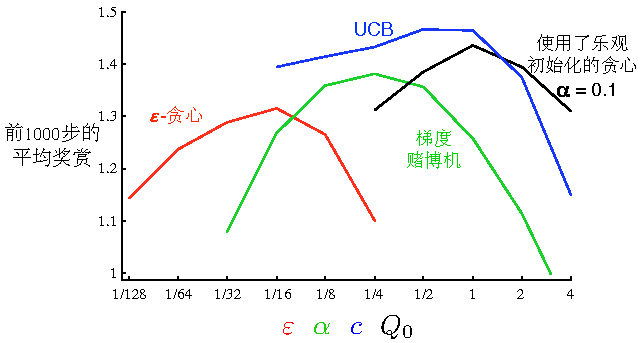
\includegraphics[width=.75\textwidth]{c2/img/figure2-6.pdf}
\caption{一份对本章中出现的各个方法的参数审视. 每一点都是特定算法与特定参数下的, 1000步奖赏的均值.}\label{fig:2.6}
\end{figure}

那么很自然地就要问这些方法中哪一个是最好的. 虽然这个问题整体上而言很难回答, 但我们显然可以在贯穿了本章的10-摇臂测试工具上使用各个方法, 并比较各自的表现. 一个困难之处是各个方法都有一个参数; 为了得到一个有意义的比较, 我们不得不将各个方法的表现作为自身参数的函数来对待. 至今为止, 我们所作的图展示了每一算法与每一参数下, 随时间变化的学习过程, 来产生在该算法与该参数设定下的\emph{学习曲线}<learning curve>. 如果我们为所有算法的所有参数设定绘制学习曲线, 那么所绘制的图将过于复杂与臃肿, 而无法产生清晰的比较. 作为代替, 我们可以使用其1000步上的平均值来代替完整的学习曲线; 这一值同学习曲线下的面积成正比. \figref{2.6}展示了本章中各个算法的这一度量, 且每一方法的度量都是各自参数的函数, 各参数使用如x轴所示的统一的标度. 这类图被称为\emph{参数审视}<parameter study>. 请注意参数值以2为因子倍增, 以对数的标度进行呈现. 也请注意各个算法的表现中极具特色的倒U形: 所有的方法在使用居中的参数值时表现最好, 即参数值既不能太大, 也不能太小. 在评估一个方法时, 我们不仅需要关注其在最佳参数设定下的表现, 也需要关注其对参数值的敏感程度. 所有的这些算法都相当不敏感, 都在一个量级的参数范围内都表现得很好. 总体而言, 在这个问题上UCB看上去表现最佳.

虽然都很简单, 但在我们看来本章中呈现的这些方法都可以算是先进水准. 虽然有更加精细的方法, 但对我们真正关注的完整强化学习问题而言, 其复杂性与所作的假设使得其不切实际. 从\chapref{5}开始, 我们将呈现用于解决完整强化学习问题的学习方法, 这些方法中就部分使用了本章中探讨的简单方法.

虽然本章中探讨的方法可能是我们目前所能做到的最好的, 但这些远不是``平衡探索与利用''这一问题的令人完全满意的解决方案.

一种经过透彻研究的, 用于平衡$k$-摇臂赌博机问题中的探索与利用的方法, 是计算一种被称为\emph{基廷斯指数}<Gittins index>的特殊动作值. 在一些重要的特殊情形下,  其在计算上易于处理, 并且可以直接计算出最优解, 但是其需要关于问题先验分布的完整知识, 而这些知识我们通常假设为是无法得到的. 此外, 无论是此方法的理论, 还是其计算上的易处理性, 都无法泛化到我们在本书的余下部分中考虑的完整强化学习问题上.

基廷斯指数方法是\emph{贝叶斯}<Bayesian>方法的一个实例. 贝叶斯方法会假设一个已知的在动作值上的初始分布, 然后在每一步后即更新该分布(假设真实的动作值是固定性的). 一般而言, 对更新的计算十分复杂,  但对于一些特定的分布(称为共轭先验<conjugate prior>)而言, 计算较为简单. 进行更新之后, 一种可行的手段是, 在每一步根据各个动作成为最优动作的后验概率来进行动作选择. 这一方法有时也被称为\emph{后验采样}<posterior sampling>或\emph{汤普森采样}<Thompson sampling>, 其通常和本章之前呈现的无分布方法<distribution-free method>中最好的那些在表现上类似.

在贝叶斯设定下, 即使想要计算探索与利用之间的\emph{最佳}平衡也是可能的. 我们可以为每一个可能的动作, 计算其所有可能的立即奖赏的概率, 以及作为结果的关于动作值的后验分布. 这一以上述方式不断行进的分布, 成为了该问题的\emph{信息状态}<information state>. 给定一定的步数, 例如1000步, 我们可以考虑所有可能的动作, 所有可能的作为结果的奖赏, 所有可能的下一动作, 所有的下一奖赏, 以此类推直到第1000步. 在这样的假设下, 所有可能的事件链的奖赏与概率都可以被确定, 我们只需要选择最佳的即可. 但是可能性树会急剧生长, 即使只有两种动作与两种奖赏, 树也会有$2^{2000}$个树叶.一般而言, 要真正进行如此大量的计算是不切实际的, 但是也许有高效的近似方式. 这一方法实际上将赌博机问题转换为了完整强化学习问题的实例. 最后, 也许我们能够使用\partref{2}中介绍的近似强化学习方法来获得这个最优解. 但这属于一个研究的课题, 超出了导论性质的本书的范畴.

% ----------------------------------- bib ---------------------------------------------
\section{参考文献与历史沿革}

暂不译.
\chapter{有限马尔科夫决策过程}\label{chap:3}

在本章中我们将介绍正式的有限卡尔科夫决策过程<finite Markov decision process, finite MDP>问题, 该问题正是我们在本书的余下部分中试图解决的. 这一问题即涉及到如赌博机问题中的评估性反馈, 又涉及到关联方面——在不同的情形下选择不同的动作. MDP\footnote{即使原文中MDP为复数, 即MDPs, 在译文中还是根据中文的语法, 不区分单复数, 仅写为MDP. 译者注.}是对系列决策过程的典型形式化, 其中动作不仅影响立即的奖赏, 也会影响此后的情形或者说是状态, 再以此影响未来的奖赏. 因此MDP涉及到延迟的奖赏, 需要就立即的奖赏与延迟的奖赏进行权衡. 在赌博机问题中, 我们评估每个动作$a$的值$q_*(a)$, 而在MDP中, 我们估计在各个状态$s$中各个动作$a$的值$q_*(s, a)$, 或者我们估计在最优动作选择下的各个状态的值$v_*(s)$. 这些依赖状态的量, 对于准确地将长期结果的赞誉<credit>分配给各个动作选择来说是必不可少的.

MDP是对强化学习问题进行的一种数学上的理想化, 可以在其中进行清晰的理论陈述. 我们将介绍强化学习问题的数学结构中的各个关键元素, 例如回报<return>, 值函数<value function>以及贝尔曼方程<Bellman equation>. 我们将尝试说明可以形式化为有限MDP的应用的范围之广. 正如整个人工智能领域, 此处也存在着应用的广度与数学上的易处理性这一对矛盾. 在本章中我们将会介绍这一对矛盾, 并讨论其中的一些权衡以及该矛盾所预示的挑战. 一些超出了MDP的强化学习方法将在\chapref{17}中被介绍.

% ----------------------------------- sec3.1 ---------------------------------------------
\section{代理-环境接口}\label{sec:3.1}

MDP意图成为``从与环境的交互中学习来达成目标''这一问题的直截了当的框架. 学习器以及决策者被称为\emph{代理}<agent>. 由代理之外的一切组成的、代理所交互的事物, 被称为\emph{环境}<environment>. 两者持续进行交互: 代理选择动作, 然后环境对动作做出反馈并将新的情形呈现给代理.\footnote{我们使用术语\emph{代理}、\emph{环境}以及\emph{动作}, 而非工程学中的术语\emph{控制器}<controller>, \emph{受控系统}<controlled system>(或\emph{设备}<plant>)以及\emph{控制信号}<control signal>, 因为前者所面向的受众更广.} 环境也给出了奖赏——代理希望通过动作选择来最大化积累量的、特殊的实数值. 

\begin{figure}[ht]
\centering
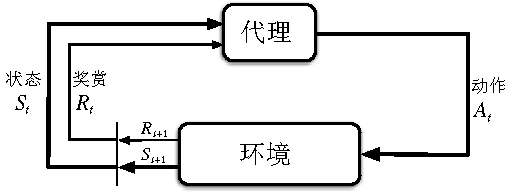
\includegraphics[width=.75\textwidth]{c3/img/figure3-1.pdf}
\caption{在马尔科夫决策过程中的, 环境与代理之间的交互.}\label{fig:3.1}
\end{figure}

% bib
更具体地说, 环境与代理在一系列离散的时步, $t = 0$, $1$, $2$, $3$, $\dots$\footnote{我们将注意力集中到离散时间序列这一情形上, 来使问题尽可能简单, 但许多概念可以拓展到连续时间的情形下(例如, 可以参见\cite{Bertsekas1996, Doya1996}).}, 上进行交互. 在每一时步$t$, 代理会接收到环境的\emph{状态}<state>$S_t \in \mathcal{S}$的某些表征, 并在此基础上选择一个\emph{动作}<action>$A_t \in \mathcal{A}(s)$\footnote{为了简化标记, 有时候我们假设在所有的状态上动作集是相同的, 并简单地将其写作$\mathcal{A}$.}. 在下一个时步, 某种程度上作为动作的结果, 代理会接收到一个实数型\emph{奖赏}<reward>$R_{t + 1} \in \mathcal{R} \subset \mathbb{R}$, 并发现自身处于一个新的状态$S_{t + 1}$中.\footnote{我们使用$R_{t + 1}$而非$R_t​$, 来表示这一奖赏归因于$A_t​$, 因为其强调了下一奖赏与下一状态$R_{t + 1}​$与$S_{t + 1}​$是联合被确定的. 不幸的是, 两者记法都在文献中被广泛使用.} 因此MDP与代理一起产生了如下的一系列轨迹:
\begin{equation}\label{eq:3.1}
S_0, A_0, R_1, S_1, A_1, R_2, S_2, A_2, R_3, \dots
\end{equation}
在\emph{有限}MDP中, 状态集、动作集与奖赏集($\mathcal{S}, \mathcal{A}, \mathcal{R}$), 都只有有限个元素. 在这一情形下, 随机变量$R_t$与$S_t$都有明确的离散概率分布, 且该分布仅依赖于前一状态与动作. 也就是说, 在给定前一状态与动作的情况下, 这两个随机变量的特定值$s' \in \mathcal{S}$及$r \in \mathcal{R}$, 出现的概率为:
\begin{equation}\label{eq:3.2}
p(s', r \mid s, a) \doteq \Pr (S_t = s', R_t = r \mid S_{t - 1} = s, A_{t - 1} = a),
\end{equation}
其适用于所有的$s', s \in \mathcal{S}, r \in \mathcal{R}, a \in \mathcal{A}(s)$. 函数$p$定义了MDP的\emph{动态}<dynamics>. 等式中等号上的点提醒我们这是一个定义式(在此情况下即为对函数$p$的), 而非由先前的定义推导出的事实. 动态函数$p : \mathcal{S} \times \mathcal{R} \times \mathcal{S} \times \mathcal{A} \rightarrow [0, 1]$, 是有4个参数的、一般的确定性函数. 其中的`$\mid$'为来自于条件概率的符号, 但在这里其仅用于提醒我们: $p$指明了各个$s$与$a$所带来的概率分布, 且
\begin{equation}\label{eq:3.3}
\sum_{s' \in \mathcal{S}} \sum_{r \in \mathcal{R}} p(s', r \mid s, a) = 1, \text{ 对所有的}s \in \mathcal{S}, a \in \mathcal{A}(s).
\end{equation}

在\emph{马尔科夫}决策过程中, 由$p$给出的概率可以完全确定环境的动态. 也就是说, $S_t$和$R_t$各个值的概率只由前一个状态与动作, 即$S_{t - 1}$和$A_{t - 1}$的具体值决定, 而不受更早的状态或动作任何影响. 最好不要将此视为决策过程上的约束, 而是视为\emph{状态}上的约束. 状态必须包括``过去代理与环境的交互中所有能对未来产生影响的方面''的信息. 如果符合此条件, 那么我们称这样的状态拥有\emph{马尔科夫性质}<Markov property>. 我们在整本书中都假设如此的马尔科夫性质, 虽然从\partref{2}开始我们将会学习不依赖于该性质的近似方法, 然后在\chapref{17}中我们将会阐述如何从非马尔科夫观测中, 学习并构建得马尔科夫状态.

从拥有4个参数的动态函数$p$中, 我们可以计算出任何和环境有关的想要的信息, 如\emph{状态转移概率}<state-transition probability>(虽然有滥用符号的嫌疑, 但我们使用有3个参数的函数$p: \mathcal{S} \times \mathcal{S} \times \mathcal{A} \rightarrow [0, 1]$来表示它),
\begin{equation}\label{eq:3.4}
p(s' \mid s, a) \doteq \operatorname{Pr}\{ S_t = s' \mid S_{t - 1} = s, A_{t - 1} = a \} = \sum_{r \in \mathcal{R}}p(s', r \mid s, a).
\end{equation}
我们可以计算出状态-动作对的期望奖赏, 并使用有2个参数的函数$r: \mathcal{S} \times \mathcal{A} \rightarrow \mathbb{R}$表示:
\begin{equation}\label{eq:3.5}
r(s, a) \doteq \mathbb{E}[R_t \mid S_{t - 1} = s, A_{t - 1} = a] = \sum_{r \in \mathcal{R}}r\sum_{s' \in \mathcal{S}}p(s', r \mid s, a),
\end{equation}
以及可以计算出针对状态--动作--下一状态三元组的期望奖赏, 并使用有3个参数的函数$r: \mathcal{S} \times \mathcal{A} \times \mathcal{S} \rightarrow \mathbb{R}$来表示:
\begin{equation}\label{eq:3.6}
r(s, a, s') \doteq \mathbb{E}[R_t \mid S_{t - 1} = s, A_{t - 1} = a, S_t = s'] = \sum_{r \in \mathcal{R}} r \frac{p(s', r \mid s, a)}{p(s' \mid s, a)} 
\end{equation}
在本书中, 我们常常使用\eqref{eq:3.2}中有4个参数的函数$p$, 但为了方便偶尔也使用其他的这些标记法.

MDP框架抽象而灵活, 可以以许多不同的方式应用到许多不同的问题中. 例如, 时步并不一定指代实际时间中的固定时间间隔; 其可以用于指代任意相继的关于决策与动作的场景. 动作可以是低层次的控制, 如加到机械臂的马达上的电压, 也可以是高层次的决策, 例如是否要吃午饭或是否去读研究生. 类似的, 状态也可以有各种各样的形式. 其可以完全由低层次的感知确定, 如传感器上的直接读数; 其也可以更加抽象且属于更加高层次, 例如对室内物体的符号性描述. 组成状态的事物可以基于对过去感知的记忆, 甚至可以完全是精神上的或主观的. 例如, 一个代理可以处于``不确定某物的位置''这么一个状态中, 或者可以从一个明确定义的角度``被吓了一跳''. 类似地, 一些动作也可以是精神上的或计算性的. 例如, 可能有一些动作可以控制代理思考的内容, 或控制代理的关注点. 一般来说, 动作可以是任何我们希望学得如何决策的决定, 而状态可以是任何我们认为可以帮助决策的事物. 

特别地, 代理与环境之间的界限, 通常不像机器人或动物体的物理界限那样. 通常来说, 该界限要近于物理界限. 例如, 机器人中的马达、机械联动装置以及传感硬件, 通常被认为是环境的一部分, 而非代理的一部分. 类似地, 如果我们将MDP框架用于人体或动物体, 肌肉、骨骼以及感知器官应该被认为是环境的一部分. 此外, 假设上说奖赏是在自然或人工学习系统的物理实体内部被计算, 但通常被认定为在代理的外部.

我们所遵循的一般规则为: 如果某物不能被代理任意改变, 那么该物被认为是在代理的外部, 因此也是环境的一部分. 我们并没有假设环境中的一切事物对于代理而言是未知的. 例如, 代理常常知道大量的关于``奖赏是怎样以一个动作与采取动作所在的状态的函数的形式被计算''的信息. 但我们总是认为奖赏的计算位于代理的外部, 因为其定义了代理所面对的任务, 因此代理没有对其进行任意修改的能力. 事实上, 在一些情况下, 代理可能知道环境运作的\emph{一切信息}, 但其面临的强化学习任务仍然非常困难, 例如我们完全知道魔方等谜题的规则, 但我们仍然无法解决它们. 代理与环境间的边界代表了代理的\emph{绝对控制能力}的限度, 而非其知识的限度.

代理与环境间的边界可以因不同的目的而置于不同的位置. 在一个复杂的机器人中, 可能有许多不同的代理同时进行操作, 而每一个都有其自身的边界. 例如, 一个代理做出了高层次的决策, 而这些高层次的决策组成了低层次的代理所面临的状态的一部分, 且正是由这些低层次的代理来实现高层次的决策. 实践中, 一旦特定的状态、动作与奖赏被选定, 代理与环境间的界限就确定下来了, 因此也确定了兴趣所在的特定决策任务.

MDP框架是对以目标为导向的、从交互中学习的问题的大幅度的抽象. 其指明——无论传感器、内存及控制装置的细节如何, 无论想要达到的目标是什么, 任何``学得目标导向的行为''这一问题可以简化为来回传递于代理与环境间的3个信号: 一个信号用于表示代理所做的决定(动作), 一个信号用于表示做出决定的基础(状态), 一个信号用于界定代理的目标(奖赏). 虽然这一框架不足以表示所有的决策问题, 但其已被证明能广泛地被应用.

当然, 不同任务中具体的状态与动作可能有巨大的差异, 且如何表示状态与动作可能会极大地影响性能. 在强化学习中, 就像在其他种类的学习中一样, 这样的关于表示的选择更像艺术而非科学. 在本书中, 我们会就``如何以好的方法来表示状态与动作''给出一些建议与例子, 但我们主要的关注点在于表示方式被选择后, 如何进行学习的一般准则.

\begin{exam}[例3.1 生物反应器]
假设强化学习用于决定生物反应器(用于产生有用的化学物质的一大堆营养物与细菌)中各个时刻的温度与搅拌速率. 在这样的一个应用中, 动作可以为控制目标温度与搅拌速率, 而控制是通过低层次的控制系统轮流激活加热元件或马达来实现的. 状态可以为(也许有延迟或经过了滤波的)热电偶以及其他传感器的读数, 连同代表桶中的原料与目标化学物质的符号性输入. 奖赏可以为生物反应器中各个时刻有用的化学物质产生的速率. 请注意其中每一个状态是传感器读数与符号性输入的列表或向量, 每一个动作是包含了目标温度与搅拌速率的向量. 对强化学习任务而言, 状态与动作拥有结构化的表示是很典型的. 而奖赏常常为单个数值.
\end{exam}

\begin{exam}[拾置机器人]
让我们考虑将强化学习用于控制反复的拾取-放置任务中机械臂的运动. 如果我们想要使机械臂学得快速而平滑的运动方式, 学习代理必须要能直接地控制马达, 且可以获得低延迟的关于机械联动装置当前的位置与速度的信息. 在这种情况下, 动作可能为加在机械臂的各个关节处的电压, 状态可能为各个关节的角度与速度的最新的读数. 如果一个物体被正确拾取并放置, 那么奖赏可以为+1. 为了激励平滑的动作, 可以在每一时步给出一个较小的负值奖赏, 并且该奖赏为运动的实时``颠簸度''的函数.
\end{exam}

\begin{exer}
写出3个适合于MDP框架的任务示例, 并给出各自的状态、动作与奖赏. 尽可能使3个示例有较大的差异. MDP框架抽象而灵活, 可以以多种方式使用. 在至少一个实例中以某种方式逼近MDP框架的极限.
\end{exer}

\begin{exer}
MDP框架足以表示\emph{所有}的目标导向的学习任务吗? 你可以想出任何明确的反例吗?
\end{exer}

\begin{exer}
现在考虑关于驾驶的问题. 你可以从油门、刹车和方向盘的角度, 即从身体与汽车的接触的角度, 来定义动作. 或者你可以从更为外侧的角度来定义动作——例如从轮胎的橡胶与路面的接触的角度看, 将动作设定为控制轮胎的扭矩. 或者你也可以从更为内侧的角度来定义动作——例如从大脑与身体的交互的角度看, 将动作定义为收缩肌肉以控制四肢. 或者你可以从相当高层次的角度看, 将动作定义为对驶向\emph{何处}的选择. 应该在哪一个层次或哪里对划定代理与环境的界限? 有没有偏好某一划分的根本理由, 或者说是可以随意选择?
\end{exer}

\hypertarget{exam:3.3}{}
\stepcounter{examcnt}%
\begin{mathbox}{例\theexamcnt: 回收机器人}
有一个在办公室中收集汽水罐的移动机器人. 该机器人有用于发现汽水罐的传感器, 以及用于拾取汽水罐并将汽水罐置于携带的垃圾箱中的机械臂与夹子; 其使用可充电电池. 该机器人的控制系统有用于理解传感信息、用于导航以及用于控制机械臂与夹子的组件. 基于电池的当前电量, 强化学习代理做出如何搜索汽水罐这样的高层次决定. 举一个简单的例子, 假设仅有两种电量等级可以被区分, 这两者组成了一个简单的状态集$\mathcal{S} = \{ \mathtt{high, low} \}$. 在每一个状态中, 代理可以决定是(1)积极地在一段时间内\texttt{搜索}<\texttt{search}>汽水罐, 或是(2)保持静止并\texttt{等待}<\texttt{wait}>别人过来扔汽水罐, 还是(3)返回据点并对电池进行\texttt{充电}<\texttt{recharge}>. 当电量等级为\texttt{high}时, 进行充电是一件愚蠢的事, 所以我们不将其包括在该状态的动作集中. 因此动作集为$\mathcal{A}(\mathtt{high}) = \{ \mathtt{search, wait} \}$以及$\mathcal{A}(\mathtt{low}) = \{ \mathtt{search, wait, recharge} \}$.

在多数时间内奖赏为0, 但是当机器人获得了一个空罐时其为正值, 当电量耗尽则其为一个绝对值较大的负值. 发现汽水罐的最好的方法就是积极地进行搜索, 但这会消耗机器人的电量, 而等待则不会消耗电量. 当机器人在搜索时, 有电量耗尽的可能. 如果电量耗尽, 那么机器人必须停机并等待援助(产生一个负奖赏). 如果电量等级为\texttt{high}, 那么机器人总是可以进行一段时间的积极搜索而没有电量耗尽的风险. 如果起始电量等级为\texttt{high}, 在经过一段时间的搜索后, 电量等级以$\alpha$的概率维持在\texttt{high}, 而以$1 - \alpha$的概率减为\texttt{low}. 在另一方面, 如果起始电量等级为\texttt{low}, 那么在经过一段时间的搜索后, 电量等级以$\beta$的概率维持在\texttt{low}, 而以$1 - \beta$的概率耗尽. 在后一种情况下, 机器人必须等待援助, 且电量在充电后恢复为\texttt{high}. 机器人收集的每个汽水罐都会产生单位奖赏, 而当机器人必须被援助时, 会产生$-3$的奖赏. 让我们使用$r_{\mathtt{search}}$和$r_{\mathtt{wait}}$(其中$r_{\mathtt{search}} > r_{\mathtt{wait}}$)来分别表示搜索与等待可以获得的汽水罐的期望数量(因此也是奖赏的期望值). 最后, 假设在机器人回据点的路上或机器人电量耗尽时, 其不能收集任何汽水罐. 那么这一系统就成为了有限MDP, 我们可以获得转移概率与期望的奖赏, 其中动态如下表所示:

\begin{center}
\begin{minipage}[c]{.5\textwidth}
\includegraphics[width=\textwidth]{c3/img/dynamics_table.pdf}
\end{minipage}
\quad
\begin{minipage}[c]{.45\textwidth}
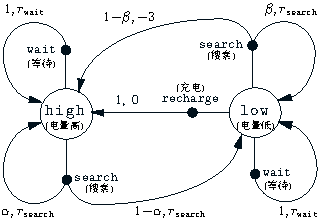
\includegraphics[width=\textwidth]{c3/img/mdp.pdf}
\end{minipage}
\end{center}
\vspace{.5em}

当前状态$s$, 动作$a \in \mathcal{A}(s)$, 及下一个状态$s'$的每一种可能的组合都对应于表中的一行. 另一种概括有限MDP动态的有用工具为如上所示的\emph{转移图}<transition graph>. 其中有两种结点: \emph{状态结点}与\emph{动作结点}. 每一个可能的状态都对应于一个状态结点(使用状态名标记的大的白圈), 每一个状态-动作对都对应于一个动作结点(连接到状态结点的、由动作名标记的小的实心圈). 于状态$s$采取动作$a$, 对应于转移图就是从状态结点$s$开始沿线移动到动作结点$(s, a)$. 然后环境通过离开动作结点$(s, a)$的箭头之一来做出响应并转移到下一个状态状态. 每一个箭头都对应于一个三元组$(s, s', a)$, 其中$s'$是下一个状态, 然后我们使用转移概率$p(s' \mid s, a)$以及该转移的期望奖赏$r(s, a, s')$来对箭头进行标记. 请注意所有离开同一个动作结点的箭头上标注的转移概率的和一定为1.
\end{mathbox}

\begin{exer}
类比于\hyperlink{exam:3.3}{例3.3}中的表, 绘制针对$p(s', r \mid s, a)​$的表格. 该表应该有$s​$, $a​$, $s'​$, $r​$以及$p(s', r \mid s, a)​$这些列, 并且每一个$p(s', r \mid s, a) > 0​$的四元组都应该有对应的行.
\end{exer}

% ----------------------------------- sec3.2 ---------------------------------------------
\section{目标与奖赏}\label{sec:3.2}

在强行学习中, 代理的目的或目标是使用一个特殊的被称为\emph{奖赏}<reward>的信号来形式化的, 且该信号由环境传给代理. 在每一时步, 奖赏就是简单的一个数值, $R_t \in \mathbb{R}$. 不那么正式地说, 代理的目标就是最大化接受到的奖赏总量. 这意味着不是最大化立即奖赏, 而是最大化长期的累积奖赏. 我们可以将这一非正式的理念阐述为\emph{奖赏假定}<reward hypothesis>:
\begin{quote}
我们所说的目标或目的可以完全被理解为: 最大化收到的标量信号(称为奖赏)的累积量的期望值.
\end{quote}
使用奖赏信号来形式化目标的概念, 是强化学习最显著的特征之一.

虽然使用奖赏信号来形式化目标可能初看上去颇具有局限性, 但在实践中其已被证明灵活且广泛可用. 来展示这一点的最好方法就是考虑一些此方法曾被如何使用或能被如何使用的例子. 例如, 为了使机器人学会走路, 研究者设定在每一时步给予正比于机器人前向移动距离的奖赏. 为了使机器人学得如何从迷宫中逃脱, 在逃离前的每个时步中奖赏都是$-1$: 这激励机器人尽快逃脱. 为了使机器人学得如何发现并收集空汽水罐以回收利用, 我们可以在多数的时间下给予其0的奖赏, 而其每收集一个汽水罐, 就给予其$+1$的奖赏. 我们也可以在机器人撞到东西或被人责骂时给予其负值的奖赏. 为了使代理学会玩西洋跳棋或国际象棋, 一个自然的选择就是获胜时给予$+1$的奖赏, 失败时给予$-1$的奖赏, 而在平局时或下棋过程中给予0的奖赏.

你可以看到在这些例子中所发生的事情. 代理总是以最大化奖赏为目标进行学习. 如果我们希望代理为我们做些什么, 我们必须以这样的原则为其提供奖赏——通过最大化累积奖赏代理能达成我们的目标. 因此, 我们设定的奖赏能否真实反映我们我们希望达成的目标就显得至关重要了. 特别来说, 奖赏信号不是将\emph{怎样}达成目标的先验知识传递给代理的地方.\footnote{更好的引入此类先验知识的地方在初始策略之处, 初始值函数之处, 或能影响这两者的地方.} 例如, 下棋代理只有在真正获胜的时候才能获得奖赏, 而不能在达成例如``吃掉了对手的棋子''或``占据了棋盘的中间位置''之类的子目标时获得奖赏. 如果在达成这类子目标时获得了奖赏, 那么代理有可能寻得达成了子目标、却没有达成真正的目标的方式. 例如, 代理可能吃了对手的棋子, 但代价是失去了比赛. 通过奖赏信号的方式, 你告诉代理你希望其达成\emph{什么}目标, 而不是你希望其\emph{如何}达成目标.

% ----------------------------------- sec3.3 ---------------------------------------------
\section{累积奖赏与分节}\label{sec:3.3}

迄今为止, 我们已经非正式地讨论了学习的目标. 我们说过代理的目标就是从长期而言, 最大化其接收的累积奖赏. 那么这怎样被正式定义呢? 如果时步$t$后接收的奖赏序列记为$R_{t + 1}$, $R_{t + 2}$, $R_{t + 3}$, $\dots$, 那么我们希望最大化这一序列的具体的哪一方面? 一般而言, 我们希望最大化\emph{期望回报}, 其中回报<return>\footnote{在余下的译文中``回报''一般为强化学习专有术语, 专指此处的return. 译者注}记为$G_t$, 被定义为奖赏序列的某一具体函数. 在最简单的情况下回报就是奖赏的和:
\begin{equation}\label{eq:3.7}
G_t \doteq R_{t + 1} + R_{t + 2} + R_{t + 3} + \dots + R_T,
\end{equation}
其中$T$为最后一个时步. 这种方式对``能自然地定义最终时步''这样的应用而言才有意义, 也就是说, 当代理与环境的交互可以自然地划分为不同的子序列时才有意义, 我们将这样的子序列称为\emph{分节}<episode>,\footnote{在文献中, 分节有时也被称为``试验''<trial>.} 例如一局比赛, 一次穿越迷宫的历程, 或任意类型的重复的交互. 每一个分节都以被称为\emph{末状态}<terminal state>的特殊状态终止, 然后重置为标准的起始状态, 或重置为对起始状态的标准分布的某一采样. 虽然分节可能以多种方式结束, 例如赢得比赛或失去比赛, 但无论上一分节是如何结束的, 紧接着的分节如何起始与此毫无关系. 因此所有的分节可以认为是在相同的末状态结束的, 只是对不同的结果而言有不同的奖赏. 具有不同分节的任务被称为分节式任务<episodic task>. 在分节式任务中, 我们有时需要将记为$\mathcal{S}$的非末状态的集合, 与记为$\mathcal{S}^+$的包括末状态的所有状态的集合区分开来. 终止的时间$T$, 通常是随分节不同而不同的随机变量

另一方面, 在许多情形下, 代理与环境的交互不能自然地划分为可辨别的分节, 而是没有限制地永远进行下去. 例如, 可以很自然地以此种方式形式化一个持续进行的过程控制任务, 或一个长生命周期的机器人应用. 我们将这样的任务称为\emph{持续式任务}<continuing task>. 对持续式任务来说, 回报公式\eqref{eq:3.7}是有问题的, 因为最终时步$T = \infty$, 且我们希望最大化的回报可以很轻易地为无穷大. (例如, 假设代理在每一时步都接收到+1的奖赏.) 因此, 本书中我们经常使用的那种回报的定义, 在概念上稍微更为复杂, 但数学上简单了很多. 

我们需要额外概念为\emph{折扣}<discount>. 据此, 代理以最大化未来接收到的折扣后奖赏的和为目标, 来进行动作选择. 特别地, 代理选择$A_t$以最大化期望的\emph{折扣后回报}:
\begin{equation}\label{eq:3.8}
G_t \doteq R_{t + 1} + \gamma R_{t + 2} + \gamma^2 R_{t + 3} + \dots = \sum_{k = 0}^{\infty} \gamma^k R_{t + k + 1},
\end{equation}
其中$0 \leq \gamma \leq 1$, $\gamma$被称为\emph{折扣率}<discount rate>.

折扣率决定了未来奖赏的当前值: 在$k$个时步后接收到的奖赏, 为立即接收到的同样的奖赏的$\gamma^{k - 1}$倍. 如果$\gamma < 1$, 那么只要奖赏序列$\{ R_k \}$是有界的, \eqref{eq:3.8}中的无限项的和就是一有限值. 如果$\gamma = 0$, 那么代理因仅关心于最大化立即奖赏而变得``短视'': 在这种情况下, 代理的目标即为选择$A_t$以仅仅最大化$R_{t + 1}$. 如果代理的每一个动作恰巧仅影响立即奖赏而不会影响未来奖赏, 那么一个短视的代理可以通过分别最大化每一个立即奖赏来最大化\eqref{eq:3.8}. 但是一般来说, 为了最大化立即奖赏而选择动作, 会减少将来的奖赏, 因而减少回报. 当$\gamma$趋近于1时, 回报的目标更多地将未来的奖赏考虑在内, 即代理的目光变得更为长远.

相邻时步中的回报彼此相关, 其相关的方式对强化学习的理论与算法来说十分重要:
\begin{equation}\label{eq:3.9}
\begin{aligned}[b]
G_t &\doteq R_{t + 1} + \gamma R_{t + 2} + \gamma^2 R_{t + 3} + \gamma^3 R_{t + 4} \dots \\
&= R_{t + 1} + \gamma (R_{t + 2} + \gamma R_{t + 3} + \gamma^2 R_{t + 4} + \dots) \\
&= R_{t + 1} + \gamma G_{t + 1}
\end{aligned}
\end{equation}
请注意如果我们定义$G_T = 0$, 那么这对所有的$t < T$的时步都成立, 即使终止发生于$t + 1$. 这使得由奖赏序列计算回报变得容易.

请注意虽然\eqref{eq:3.8}中的回报由无穷多项组成, 但如果奖赏为非0常数, 且$\gamma < 1$, 那么回报值仍是有限的值. 例如, 如果奖赏恒定为+1, 那么回报为
\begin{equation}\label{eq:3.10}
G_t = \sum_{k = 0}^{\infty} \gamma^k = \frac{1}{1 - \gamma}
\end{equation}

\begin{exer}
\secref{3.1}中的等式是针对于持续式任务的, 如果想要将其用于分节式任务中的话, 需要对其进行(非常小的)修改. 通过给出\eqref{eq:3.3}修改后的版本来证明你知道如何进行修改. 
\end{exer}

\begin{wrapfigure}[6]{r}{.45\textwidth}
\centering
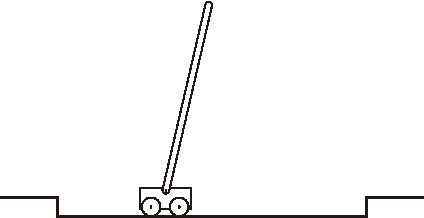
\includegraphics[width=.4\textwidth]{c3/img/pole-balancing.pdf}
\end{wrapfigure}
\mbox{}~
\begin{exam}[杆之平衡]
本任务的目标为在一个沿轨道移动的小车上施加合适的力, 使得铰接于小车上的杆子不会落倒: 如果杆子与垂直方向的夹角超过了给定值, 或小车跑出了轨道, 那么就算作失败. 每次失败后杆子都会重置到垂直方向上. 可以以分节式的方式处理该任务, 其中重复进行的将杆保持平衡的尝试, 就是自然划分的分节. 在这种情况下, 尚未失败的时步中奖赏为$+1$, 那么每一时步中的回报就是距离失败所余下的步数. 这样的话, 如果杆能永远保持平衡, 那么回报就会趋于无穷大. 作为代替, 我们可以使用折扣, 将此任务作为持续式任务对待. 在这种情况下, 每次失败时奖赏为$-1$, 而所有的其他时步中奖赏为0. 那么在每一时步中, 回报将和$- \gamma^K$相关, 其中$K$为距离失败的时步数. 无论在哪种情况下, 都是令杆尽可能长时间地保持平衡来最大化回报.
\end{exam}

\begin{exer}
假设你将杆之平衡作为分节式任务对待, 但同时也使用折扣, 且除了失败时奖赏为$-1$外, 其他所有时间奖赏为0. 那么每一时步中的回报将会是如何? 该回报将与本任务上折扣、连续式的设定下的回报有何区别?
\end{exer}

\begin{exer}
假设你在设计一个走迷宫的机器人. 你决定在其逃出迷宫时给予$+1$的奖赏, 而在所有的其他时间均给予0的奖赏. 这个任务看上去可以很自然地划分为各个分节——即相继的走迷宫的尝试——所以你决定将其作为分节式任务对待, 其中目标就是最大化期望的奖赏和\eqref{eq:3.7}. 在令代理尝试走一段时间的迷宫后, 你发现其在逃离迷宫方面没有任何改进. 哪里出错了呢? 你有没有真正地将你的目标传达给代理?
\end{exer}

\begin{exer}
假设$\gamma = 0.5$, 且接收到了如下的奖赏序列: $R_1 = -1$, $R_2 = 2$, $R_3 = 6$, $R_4 = 3$以及$R_5 = 2$, 其中$T = 5$. 那么$G_0, G_1, \dots, G_5$为多少? 提示: 从后往前算.
\end{exer}

\begin{exer}
假设$\gamma = 0.9$, 且接收到的奖赏序列为: $R_1 = 2$, 之后为无数多个7. 那么$G_1$和$G_0$的值为多少?
\end{exer}

\begin{exer}
证明\eqref{eq:3.10}中的第二个等号.
\end{exer}

% ----------------------------------- sec3.4 ---------------------------------------------
\section{分节式与持续式任务的统一标记方式}\label{sec:3.4}

在前一节我们介绍了两种强化学习任务: 一种中代理与环境间的交互可以自然地划分为独立的分节(分节式任务), 而另一种中并非如此(持续式任务). 前一种情况从数学上说更为简单, 因为每个动作仅影响该分节中随后接收到的有限个奖赏. 在本书中, 我们有时考虑一种, 有时考虑另一种, 但常常是两种一起考虑. 因此建立一种能同时精确地用于两种情形的标记方式就显得很有帮助了.

我们需要一些额外的标记来更清楚地表示分节式任务. 对于分节式任务, 我们不能将其考虑为由时步组成的单个长序列, 而是考虑为一系列的分节, 其中每一个分节都由有限的时步序列组成. 在每一个分节开始时, 我们重新从0开始对时步进行计数. 因此, 仅使用$S_t$, 即时步$t$处的状态, 来进行指代是不够的, 我们需要使用$S_{t, i}$, 即分节$i$中的时步$t$处的状态, 来进行指代(类似地, 有$A_{t, i}$, $R_{t, i}$, $\pi_{t, i}$, 以及$T_i$等等). 然而, 事实上当我们讨论分节式任务时我们几乎不用对各个分节进行区分. 我们几乎总是仅考虑单个特定分节, 或者我们所论述的对所有的分节都成立. 因此, 实践中我们总是轻微地滥用标记: 省去了分节的具体索引. 也就是说, 我们使用$S_t$时, 我们指的是$S_{t, i}$, 其余的也类似.

为了得到分节式与持续式任务的统一标记方式, 我们还需要另一个规约. 在情形\eqref{eq:3.7}下, 我们将回报定义为有限个项的和; 而在情形\eqref{eq:3.8}下, 我们将其定义为无限个项的和. 如果我们将分节的终结视为进入了一个特殊的\emph{吞没状态}<absorbing state>, 即仅转移到自身且获得的所有奖赏均为0的状态, 那么我们可以将两种任务统一起来. 例如, 考虑如下的转移图:

\begin{figure}[ht]
\centering
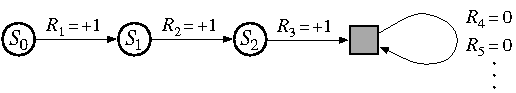
\includegraphics[width=.7\textwidth]{c3/img/transition_graph.pdf}
\end{figure}

其中实心的方框表示对应于分节的终止的、特别的吞没状态. 从$S_0$开始, 我们获得了奖赏序列$+1$, $+1$, $+1$, $0$, $0$, $0$, $\dots$. 那么仅对前$T$个奖赏求和的值(此处$T = 3$), 同对整个无穷项的序列求和的值是一样的. 即使我们引入折扣, 这同样成立. 因此, 我们可以以如下方式定义一般性的回报: 依据于式\eqref{eq:3.8}; 并且依照``当不需要分节的编号时将其省略"这一惯例; 同时如果和有定义, 那么保留$\gamma = 1$的可能(例如, 如果所有的分节都会终止, 那么可以这么做). 作为代替, 我们可以获得
\begin{equation}\label{eq:3.11}
G_t \doteq \sum_{k = t + 1}^{T} \gamma^{k - t - 1} R_k,
\end{equation}
其中$T= \infty$或$\gamma = 1$都是被允许的(但不能两者同时). 我们在的本书的余下内容中使用这一惯例, 以简化标记并展示分节式任务与持续式任务的高度并行性. (更晚些, 在\chapref{10}中, 我们将介绍连续且非折扣的表述方式.)

% ----------------------------------- sec3.5 ---------------------------------------------
\section{策略与值函数}\label{sec:3.5}

几乎所有的强化学习算法都涉及到对值函数——估计对代理而言给定状态的\emph{好坏程度}的, 以状态为参数的函数(或估计在给定状态执行给定动作的好坏程度的, 以状态-动作对为参数的函数)——进行估计. 这里``好坏程度"的概念是就可以期待的未来奖赏定义的, 或更准确地说, 就期望回报定义的. 当然, 代理所期望的能在未来接收到的奖赏, 依赖于其所采取的动作. 因此, 值函数被定义为同具体的采取动作的方式——即策略——相关.

正式地说, \emph{策略}<policy>是从状态到选择各个可能动作的概率的映射. 如果代理在时步$t$使用策略$\pi$, 那么$\pi(a \mid s)$即为当$S_t = s$时$A_t = a$的概率. 就像$p$一样, $\pi$也是一个普通的函数; $\pi(a \mid s)$中的``$\mid$"仅用于提醒我们: 该函数为每一个$s \in \mathcal{S}$定义了$a \in \mathcal{A}(s)$上的概率分布. 由强化学习方法指定代理的策略如何根据经历来调整.

\begin{exer}
如果当前状态为$S_t$, 并且根据概率性策略$\pi$来进行动作选择, 那么如何用$\pi$以及4参数的函数$p$\eqref{eq:3.2}来表示$R_{t + 1}$的期望值?
\end{exer}

在策略$\pi$下状态$s$的值函数, 记为$v_\pi(s)$, 为从状态$s$开始, 并在之后遵循策略$\pi$, 而获得的期望回报. 对于MDP, 我们可以用下式正式定义$v_\pi$:
\begin{equation}\label{eq:3.12}
v_\pi(s) \doteq \mathbb{E}_\pi[G_t \mid S_t = s] = \mathbb{E}_\pi \left[ \sum_{k = 0}^{\infty} \gamma^k R_{t + k + 1} \mid S_t = s \right], \text{对所有的}s \in \mathcal{S},
\end{equation}
其中$\mathbb{E}_\pi [\cdot]$表示当代理使用策略$\pi$时随机变量的期望值, 而$t$为任一时步. 如果有吞没状态的话, 那么该状态的值一定为0. 我们将函数$v_\pi$称为\emph{针对策略$\pi$的状态值函数}<state-value function>. 

类似的, 我们将策略$\pi$下在状态$s$中采取动作$a$的值, 定义为从状态$s$开始, 采取动作$a$, 并在之后遵循策略$\pi$, 而可以获得的期望回报, 并将其记为$q_\pi(s, a)$:
\begin{equation}\label{eq:3.13}
q_\pi(s, a) \doteq \mathbb{E}_\pi[G_t \mid S_t = s, A_t = a] = \mathbb{E}_\pi \left[ \sum_{k = 0}^{\infty} \gamma^k R_{t + k + 1} \mid S_t = s, A_t = a \right].
\end{equation}
我们将$q_\pi$称为\emph{针对策略$\pi$的动作值函数}<action-value function>.

\begin{exer}
使用$q_\pi$和$\pi$来表示$v_\pi$.
\end{exer}

\begin{exer}
使用$v_\pi$和4参数函数$p$来表示$q_\pi$.
\end{exer}

值函数$v_\pi$与$q_\pi$可以利用经历来进行估计. 例如, 如果对遇到的每一个状态, 记录该状态随后的实际回报, 然后计算均值, 那么当遇到该状态的次数趋于无穷大时, 均值也会收敛到该状态的值$v_\pi(s)$. 如果对每一个状态中的各个动作分别计算均值, 那么这些均值也会类似地收敛到$q_\pi(s, a)$. 我们将此类估计方式称为\emph{蒙特卡洛方法}<Monte Carlo method>, 因为此类方法涉及到对大量实际回报值的随机样本进行平均. 此类方法将会在\chapref{5}中进行介绍. 当然, 如果有许多状态的话, 那么为每个状态各自维持一个均值是不切实际的. 作为代替, 代理将以参数化函数的形式(参数个数必须少于状态个数)来维持$v_\pi$与$q_\pi$, 并调整参数来更好地与观测到的回报匹配. 这样也可以产生精确的估计值, 但这极其依赖于参数化函数近似器的种类. 这些内容将在本书的\partref{2}讨论.

一条贯穿于强化学习与动态规划始终的, 关于值函数的基本性质为: 其满足类似于我们已经讨论过的回报公式\eqref{eq:3.9}那样的递归关系. 对任意策略$\pi$和任意状态$s$来说, 下述的一致性条件在$s$的值与其可能的后一状态的值间成立:
\begin{align}
v_{\pi}(s) &\doteq \mathbb{E}_{\pi}[G_t \mid S_t = s] \nonumber\\
&= \mathbb{E}_{\pi}[R_{t + 1} + \gamma G_{t + 1} \mid S_t = s]  \tag*{\text{通过$\eqref{eq:3.9}$}}\nonumber\\
&= \sum_a \pi(a \mid s) \sum_{s'}\sum_{r}p(s', r \mid s, a) \Big[r + \gamma \mathbb{E}_{\pi}[G_{t + 1} \mid S_{t + 1} = s'] \Big]  \nonumber\\
&= \sum_a \pi(a \mid s) \sum_{s', r}p(s', r \mid s, a)\Big[ r + \gamma v_{\pi}(s') \Big], \text{ 对所有的} s \in \mathcal{S}, \label{eq:3.14}
\end{align}
且其中隐含着以下几点: 动作$a$来自于集合$\mathcal{A}(s)$, 下一状态$s'$来自于集合$\mathcal{S}$(在分节式问题中来自集合$\mathcal{S}^+$), 奖赏$r$来自于集合$\mathcal{R}$. 请注意在最后一个等式中, 我们是怎么将两个和式——一者为在$s'$的所有值上求和, 另一者为在$r$的所有值上求和——归并到对两者的所有可能值求和. 我们常常使用这种归并后的和式来简化公式. 也请注意对最后那个表达式, 我们可以轻易地将其作为期望值来理解. 实际上其为在三个变量$a$, $s'$与$r$的所有值上的和式. 对每一个三元组, 我们计算其概率$\pi(a \mid s)p(s', r \mid s, a)$, 并将该概率作为方括号内值的权重, 然后在所有的概率上求和来得到期望值. 

\begin{wrapfigure}{r}{.3\textwidth}
\centering
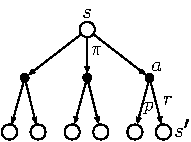
\includegraphics[width=.3\textwidth]{c3/img/backup_diagram.pdf}\\
对$v_{\pi}$的逆流图
\end{wrapfigure}
等式\eqref{eq:3.14}为\emph{针对$v_{\pi}$的贝尔曼方程}<Bellman equation>. 其阐述了某一状态的值与其各个后一状态的值间的关系. 试想下从某一个状态向前看, 看到了所有可能的后一状态的情形, 如右图所示. 每一个空心圆代表了一个状态, 而每一个实心圆代表了一个动作-状态对<state-action pair>. 从最上方的作为根结点的状态$s$出发, 代理可以基于其策略$\pi$选择某一动作集中的任何一个动作——图中展示了3个这样的动作. 从任一动作出发, 环境会反馈以数个下一状态(在图中展示了两个)中的选择, 即$s'$, 以及依据由函数$p$给出的动态得到的奖赏$r$. 贝尔曼方程\eqref{eq:3.14}以概率为权重, 在所有可能性上求和. 其显示出: 一状态的值一定等于其下一状态的(未经折扣的)值与随同的奖赏这两者之和的期望值.

值函数$v_{\pi}$是其贝尔曼方程的唯一解. 我们将在后续的章节中展示: 贝尔曼方程何以成为数种计算、近似与学习$v_{\pi}$的方法的基础. 我们将上面出现过的那种图称为\emph{逆流图}<backup diagram>, 因为其绘制出的关系构成了更新或\emph{逆流}<backup>操作的基础, 而该操作为强化学习方法的核心. 这些操作将值的信息从某一状态的后一状态(或动作-状态对), 逆向传输到该状态(或状态-动作对). 我们将在本书中持续使用逆流图, 来提供对正在讨论的算法的图形化概述. (请注意, 不像转移图, 逆流图中的状态结点并不一定表示不同的状态; 例如, 一个状态的后一状态可能为其本身.)

\hypertarget{exam:3.5}{}
\begin{exam}[网格世界]
\figref{3.2}(左)展示了一矩形的网格世界以作为有限MDP的简单示例. 网格中的每一个小格都对应于环境中的状态. 在一个小格上, 有4种可能的动作: \textbf{北移}, \textbf{南移}, \textbf{东移}, 以及\textbf{西移}, 其中各个动作都确定性地使代理在网格上沿对应的方向移动一格. 如果所采取的动作将令代理脱离网格, 那么该动作的结果为代理的位置保持不变, 且造成$-1$的奖赏. 除了上述动作与将代理移出特殊状态\textsf{A}与\textsf{B}的动作外, 其他的动作只会造成0的奖赏. 在状态\textsf{A}上, 所有的4个动作会产生$+10$的奖赏, 并将代理带至\textsf{A'}. 在状态\textsf{B}上, 所有的4个动作会产生$+5$的奖赏, 并将代理带至\textsf{B'}.

\begin{figure}[htb]
\centering
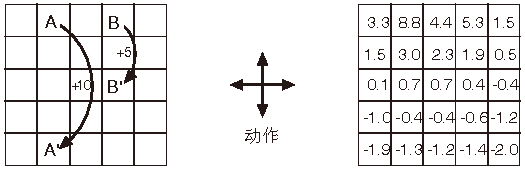
\includegraphics[width=.8\textwidth]{c3/img/figure3-2.pdf}
\caption{网格世界的例子: 例外的奖赏动态(左)与等可能性随机策略的状态值函数(右)}\label{fig:3.2}
\end{figure}

假设在所有的状态中, 代理都以相等的概率选择所有的4个动作. \figref{3.2}展示了在$\gamma = 0.9$的折扣情形下, 针对这一策略的值函数$v_{\pi}$. 此函数是通过解线性方程组\eqref{eq:3.14}得到的. 请注意在下方边界上的负值: 这是在本随机策略下代理有较大的可能撞到网格的边界所导致的结果. 状态\textsf{A}为本策略下最好的状态, 但其值小于10, 即小于其立即奖赏, 这是因为从状态\textsf{A}代理会被带至\textsf{A'}, 而在\textsf{A'}代理很可能会撞到网格的边界. 另一方面, 状态\textsf{B}的值大于5, 即大于其立即奖赏, 这是因为从状态\textsf{B}代理会被带至\textsf{B'}, 而状态\textsf{B'}的值为正. 从B开始因撞到边界而产生的期望惩罚值(负的奖赏)不及误打误撞进入\textsf{A}或\textsf{B}而产生的期望奖赏.
\end{exam}

\begin{exer}
就\examref{3.5}中\figref{3.2}(右)所示的值函数$v_{\pi}$而言, 贝尔曼方程\eqref{eq:3.14}一定对每一个状态都成立. 从数值上来证明, 就值分别为$+2.3$, $+0.4$, $-0.4$, $+0.7$的相邻状态而言, 贝尔曼方程在值为$+0.7$的正中间的状态上成立. (这些数值都只保留了1位有效数字.)
\end{exer}

\begin{exer}
在网格世界的例子中, 当离开目标状态时奖赏为正, 当撞到世界的边界时奖赏为负, 且在余下的时间内奖赏为0. 是这些奖赏的正负重要, 还是只有奖赏间的差值重要? 使用\eqref{eq:3.8}来证明向所有的奖赏加上一个常数$c$, 将会令所有状态的值增加一常数$v_c$, 因此不影响任意策略下的任意状态间的差值. 如何用$c$和$\gamma$来表示$v_c$?
\end{exer}

\begin{exer}
现在考虑在一个如走迷宫的分节式任务中, 向所有的奖赏加上一个常数$c$. 这会有什么影响, 还是像持续式任务中那样使得任务保持不变? 为什么或为什么不? 请给出一个例子.
\end{exer}


\begin{exam}[高尔夫]
\begin{figure}[htb]
\centering
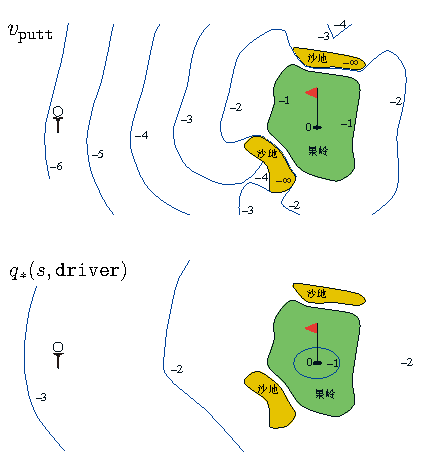
\includegraphics[width=.6\textwidth]{c3/img/figure3-3.pdf}
\caption{一个高尔夫的例子: 仅推球的状态值函数(上方)与使用木杆的最优动作值函数(下方)).}\label{fig:3.3}
\end{figure}
为了将打高尔夫球形式化为强化学习任务, 我们令每一杆都有$-1$的惩罚值(负的奖赏), 直到球进洞为止. 状态为球的位置. 状态的值为从当前位置到进洞所需的杆数的相反数. 我们的动作为如何进行瞄准与击球, 以及我们选择什么样的球杆. 让我们假定前者是给定的, 只需考虑球杆的选择, 其中我们假设要么选择推杆<\texttt{putter}>, 要么选择木杆<\texttt{driver}>. \figref{3.3}中的上半部分展示了总使用推杆时的状态值函数$v_{\mathtt{putt}}$. \emph{位于洞中}这一吞没状态值为0. 假设可以从果岭\footnote{果岭是高尔夫球运动中的一个术语, 是指球洞所在的草坪, 果岭的草短、平滑, 有助于推球. 果岭\\为英文green音译而来, 对应于\figref{3.3}中的绿色部分. 译者注.}的任意一处推球入洞; 这些状态的值为$-1$. 在果岭之外, 我们不能仅一杆就推球入洞, 因此状态值的绝对值更大. 如果我们可以靠一次推球进入果岭, 那么该状态的值一定比果岭的状态值小1, 即值为$-2$. 为了简洁起见, 让我们假设我们可以十分精确与确定性地推球, 但距离有限. 这为我们给出了图中标着$-2$的尖锐轮廓线; 所有介于该轮廓线与果岭之间的位置都需要恰好2杆来使球进洞. 类似地, 任一可以通过一次推球到达$-2$轮廓线的位置的值一定为$-3$, 并以此类推来得到图中所示的所有轮廓线. 推球并不能将球推出沙坑, 因此该状态值为$-\infty$. 总体而言, 从球座到洞我们共需要6杆. 
\end{exam}

\begin{wrapfigure}[3]{r}{.16\textwidth}
\centering
\vspace{-0.7em}
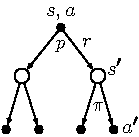
\includegraphics[width=.16\textwidth]{c3/img/action_value_backup_diagram.pdf}\\
{\tiny 针对$q_{\pi}$的逆流图}
\end{wrapfigure}
\mbox{}~
\begin{exer}
针对动作值$q_{\pi}$的贝尔曼方程是怎样的? 其中动作值$q_{\pi}(s, a)$必须用$(s, a)$的所有可能的后一动作-状态对的动作值$q_{\pi}(s', a')$来表示. 提示: 右侧的逆流图对应于这一方程. 请给出类似于\eqref{eq:3.14}的针对动作值的等式推导过程.
\end{exer}

\begin{exer}
某一状态的值依赖于该状态下可能的动作的值, 以及在当前策略下采取各个动作的可能性. 我们可以通过``以某一状态为根且考虑各个可能的动作''的逆流图来理解这一点:
\begin{center}
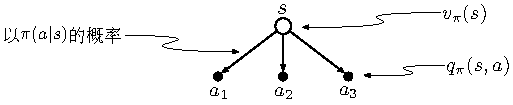
\includegraphics[width=.6\textwidth]{c3/img/state_value_ito_action_value.pdf}
\end{center}
依据这一直观感受与给出的逆流图, 请写出这样的等式: 其使用叶结点的值$q_{\pi}(s, a)$(给定$S_t = s$)来表示根结点的值$v_{\pi}(s)$. 这一等式应该包括基于策略$\pi$的期望式. 然后给出第二个等式, 其中期望式使用$\pi(a \mid s)$展开, 使得等式中没有期望符号.
\end{exer}

\begin{exer}
一个动作的值, $q_{\pi}(s, a)$, 依赖于期望的下一奖赏与期望的余下奖赏的和. 同样, 我们可以通过``以某一动作(动作-状态对)为根, 发散出各个可能的下一状态''的逆流图来理解这一点:
\begin{center}
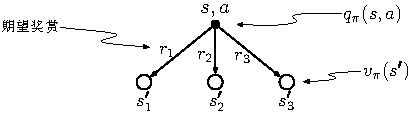
\includegraphics[width=.45\textwidth]{c3/img/action_value_ito_state_value.pdf}
\end{center}
依据这一直观感受与给出的逆流图, 请写出这样的等式: 其使用期望的下一奖赏$R_{t + 1}$与期望的下一状态的值$v_{\pi}(S_{t + 1})$(给定$S_t = s$及$A_t = a$)来表示动作值$q_{\pi}(s, a)$. 这一等式应该包括一个期望式, 但该期望式并\emph{不}基于当下策略. 然后给出第二个等式, 其中期望式使用如\eqref{eq:3.2}定义的$p(s', r \mid s, a)$来展开, 使得该等式中没有期望符号.
\end{exer}

% ----------------------------------- sec3.6 ---------------------------------------------
\section{最优策略与最优值函数}\label{sec:3.6}

粗略地说, 解决强化学习问题即意味着发现能在长期中接高额奖赏的策略. 对于有限MDP来说, 我们可以使用下述的方式精确地定义最优策略. 通过值函数, 我们可以在策略上定义一个偏序关系. 如果在所有的状态上, 使用策略$\pi$获得的期望回报都高于或等于策略$\pi'$, 则策略$\pi$被定义为优于策略$\pi'$. 换句话说, $\pi \geq \pi'$当且仅当$v_{\pi}(s) \geq v_{\pi'}(s)$对所有的$s \in \mathcal{S}$成立. 总有一个策略优于或其他的所有策略或和其他的所有策略一样好. 这就是\emph{最优策略}<optimal policy>. 虽然可能有不止一个的最优策略, 但我们将所有的最优策略都记为$\pi_{*}$. 这些最优策略都有着相同的状态值函数, 该状态值函数称为\emph{最优状态值函数}<optimal state-value function>, 记为$v_*$, 定义如下:
\begin{equation}\label{eq:3.15}
v_*(s) \doteq \max_{\pi}v_{\pi}(s),
\end{equation}
对所有的$s \in \mathcal{S}$成立.

最优策略也共享着相同的\emph{最优动作值函数}<optimal action-value function>, 其记为$q_*$, 且定义如下:
\begin{equation}\label{eq:3.16}
q_*(s, a) \doteq \max_{\pi}q_{\pi}(s, a),
\end{equation}
对所有的$s \in \mathcal{S}$与$a \in \mathcal{A}(s)$成立. 对状态-动作对$(s, a)$来说, 这一函数定义了在状态$s$下采取动作$a$, 并在之后遵循最优策略而可以获得的期望回报. 因此, 我们可以如下用$v_*$定义$q_*$:
\begin{equation}\label{eq:3.17}
q_*(s, a) = \mathbb{E}[R_{t + 1} + \gamma v_*(S_{t + 1}) \mid S_t = s, A_t = a].
\end{equation}

\begin{exam}[高尔夫的最优值函数]
\figref{3.3}的下侧展示了可能的最优动作值函数$q_*(s, \mathtt{driver})$的轮廓线. 这些值为, 如果我们先用木杆打一杆, 并在之后选择木杆或推杆两者中较好的那个, 而得到的各个状态的值. 木杆能让我们击出去的球更远, 但会损失准确度. 当使用木杆时, 只有我们离球洞足够近, 我们才能一杆入洞, 因此$q_*(s, \mathtt{driver})$的$-1$的轮廓线只覆盖了果岭的一小部分. 但如果我们能打两杆的话, 我们就可以从远得多的地方击球入洞, 就像$-2$的轮廓线所示的那样. 在这种情形下, 我们不必一直用木杆来进到较小的$-1$轮廓线内, 而只需要进到果岭内; 在那里我们可以使用推杆. 最优动作值函数给出了如下情形下的值: 先采取特定的\emph{最初}动作, 此处即为使用木杆, 之后则一直选择最佳的动作. $-3$的轮廓线是在更外围的地方, 且包括了球座. 从球座起, 最佳的动作序列为先使用两次木杆然后使用一次推杆, 这样就可以将球打入洞中.
\end{exam}

因为$v_*$为某一策略下的值函数, 其必须满足针对状态值的贝尔曼方程\eqref{eq:3.14}所给出的自洽条件. 但因为最优值函数的缘故, $v_*$的一致性条件可以以不参照任何特定策略的特殊形式写出. 这即为针对$v_*$的贝尔曼方程, 或者可以称之为\emph{贝尔曼最优性方程}<Bellman optimality equation>. 直观地看, 贝尔曼最优性方程所表述的事实为: 在最优策略下, 一个状态的值一定等于在该状态下采取最优动作所获得的期望回报:
\begin{align}
v_*(s) &= \max_{a \in \mathcal{A}(s)}q_{\pi_*}(s, a) \nonumber \\
&= \max_a \mathbb{E}_{\pi_*}[G_t \mid S_t = s, A_t = a] \nonumber \\
&= \max_a \mathbb{E}_{\pi_*}[R_{t + 1} + \gamma G_{t + 1} \mid S_t = s, A_t = a] \tag*{\text{通过$\eqref{eq:3.9}$}} \nonumber \\
&= \max_a \mathbb{E}[R_{t + 1} + \gamma v_*(S_{t + 1}) \mid S_t = s, A_t = a] \label{eq:3.18} \\
&= \max_a \sum_{s', r}p(s', r \mid s, a)[r + \gamma v_*(s')] \label{eq:3.19}
\end{align}
最后两个等式是针对$v_*$的贝尔曼最优性方程的两种形式. 针对$q_*$的贝尔曼最优性方程为
\begin{equation}\label{eq:3.20}
\begin{aligned}[b]
q_*(s. a) &= \mathbb{E} \left[ R_{t + 1} + \gamma \max_{a'}q_*(S_{t + 1}, a') \mid S_t = s, A_t = a \right] \\
&= \sum_{s', r} p(s', r \mid s, a) \left[ r + \gamma \max_{a'}q_*(s', a') \right].
\end{aligned}
\end{equation}

\figref{3.4}中的逆流图从图形上展示了针对$v_*$与$q_*$的贝尔曼最优性方程中所考虑的未来状态与动作的范围. 这些逆流图和之前呈现的针对$v_\pi$与$q_\pi$的逆流图类似, 只是在选择点处添加了添加了弧线来表明进行了最优选择, 而不是计算给定策略下的期望值. 图中左侧的逆流图从图形上表示贝尔曼最优性方程\eqref{eq:3.19}, 而右侧的从图形上表示\eqref{eq:3.20}.

\begin{figure}[htb]
\centering
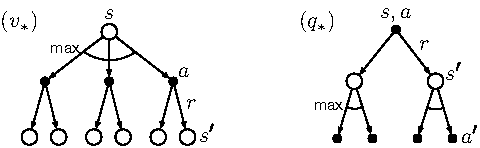
\includegraphics[width=.6\textwidth]{c3/img/figure3-4.pdf}
\caption{针对$v_*$与$q_*$的逆流图}\label{fig:3.4}
\end{figure}

对于有限MDP而言, 针对$v_*$的贝尔曼最优性方程\eqref{eq:3.19}有不依赖于策略的唯一解. 贝尔曼最优性方程实际上是方程组, 每一个状态都对应于一个方程, 因此如果有$n$个状态的话, 那么就在$n$个方程中有$n$个未知数. 如果环境的动态$p$是已知的, 那么原则上说我们可以从各种各样的解非线性方程组的方法中选择一个来求得$v_*$. 同样, 也可以解类似的方程组来求出$q_*$.

一旦我们知道了$v_*$, 那么确定最优策略就相对来说比较容易了. 对每个状态$s$来说, 都有一个或多个动作可以在贝尔曼最优性方程中取得最大值. 任何只将非零的概率分配给这些动作的策略都是最优策略. 你可以将此理解为单步搜索. 如果你已经知道了最优值函数$v_*$, 那么在单步搜索后表现得最好的动作即为最优动作. 另一个看待这一点的视角为: 任一就最优值函数$v_*$而言贪心的策略都是最优策略. 在计算机科学的领域中, 术语贪心用于``只基于局部或当前的考量来进行选择, 而不考虑这样的选择是否会在将来阻碍我们做出更好的选择''这样的搜索或决策过程. 因此, 其用于形容仅基于短期结果来进行动作选择的策略. $v_*$的优美之处在于, 如果我们将其用于对动作的短期结果进行评估——或更确切地说, 单步结果——那么从我们所关注的长期的角度看, 贪婪策略事实上是最优的, 因为$v_*$已经将所有可能的未来动作所产生的关于奖赏的影响考虑在内. 通过$v_*$, 最优的长期期望回报转为了可以在每个状态上通过局部、立即的计算而获得的量. 因此, 单步搜索即可得到长期而言最优的动作.

如果我们知道了$q_*$, 那么选择最优动作甚至可以更简单. 有了$q_*$, 代理甚至都不必进行单步搜索: 对任一状态$s$, 代理可以轻松地发现最大化$q_*(s, a)$的动作. 动作值函数实际上已经存储了所有单步搜索的结果. 其将最优的长期期望回报作为``可以在每一个状态-动作对上立即获得的本地的量''提供. 因此, 以构建动作-状态对上而非状态上的函数为代价, 最优动作值函数使得我们可以选择最优动作而不必了解任何和可能的后一状态与后一状态的值有关的信息, 即不必了解关于环境的动态的任何信息.

\begin{exam}[解决网格世界问题]
对于在\examref{3.5}中介绍的简单的网格问题, 我们将其在\figref{3.5}(左)中再次进行展示, 并假设我们已经解得了针对$v_*$的贝尔曼方程. 让我们回想一下, 紧随状态\textsf{A}的是+10的奖赏以及到状态\textsf{A'}的转移, 而紧随状态\textsf{B}的是+5的奖赏以及到状态\textsf{B'}的转移. \figref{3.5}(中)展示了最优值函数, 而\figref{3.5}(右)展示了对应的最优策略. 有些小方格内有多个箭头, 则所有这些箭头对应的动作都是最优的.
\begin{figure}[H]
\centering
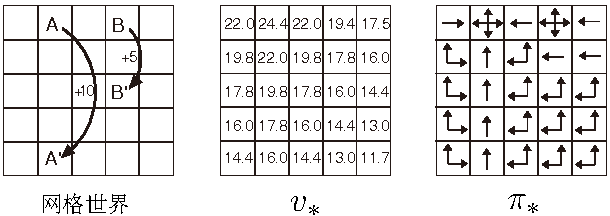
\includegraphics[width=.8\textwidth]{c3/img/figure3-5.pdf}
\caption{网格世界例子的最优解}\label{fig:3.5}
\end{figure}
\vspace{-2em}
\end{exam}

\begin{exam}[回收机器人问题上的贝尔曼最优性方程]
使用\eqref{eq:3.19}, 我们可以明确地给出回收机器人例子上的贝尔曼最优性方程. 简洁起见, 我们将状态\texttt{high}, \texttt{low}以及动作\texttt{search}, \texttt{wait}, \texttt{recharge}分别记为\texttt{h}, \texttt{l}, \texttt{s}, \texttt{w}, \texttt{re}. 因为只有两个状态, 因此贝尔曼最优性方程包含了两个方程. 针对$v_*(\mathtt{h})$的方程可以写作:
\begin{equation*}
\newcommand{\tth}{\mathtt{h}}
\newcommand{\tts}{\mathtt{s}}
\newcommand{\ttl}{\mathtt{l}}
\newcommand{\ttw}{\mathtt{w}}
\begin{aligned}[b]
v_*(h) &= \max \left.
\begin{cases}
&p(\tth \mid \tth, \tts) [r(\tth, \tts, \tth) + \gamma v_*(\tth)] + p(\ttl \mid \tth, \tts)[r(\tth, \tts, \ttl) + \gamma v_*(\ttl)], \\
&p(\tth \mid \tth, \ttw) [r(\tth, \ttw, \tth) + \gamma v_*(\tth)] + p(\ttl \mid \tth, \ttw)[r(\tth, \ttw, \ttl) + \gamma v_*(\ttl)]
\end{cases} \right\} \\
&= \max \left.
\begin{cases}
&\alpha [r_\tts + \gamma v_*(\tth)] + (1 - \alpha)[r_\tts + \gamma v_*(\ttl)], \\
&1[r_\ttw + \gamma v_*(\tth)] + 0[r_\ttw + \gamma v_*(\ttl)]
\end{cases} \right\} \\
&=\max \left.
\begin{cases}
&r_\tts + \gamma[\alpha v_*(\tth) + (1 - \alpha)v_*(\ttl)], \\
&r_\ttw + \gamma v_*(\tth)
\end{cases} \right\}.
\end{aligned}
\end{equation*}
如果$v_*(\mathtt{l})$也沿用同样的流程的话, 将得到如下的方程
\begin{equation*}
\newcommand{\tth}{\mathtt{h}}
\newcommand{\tts}{\mathtt{s}}
\newcommand{\ttl}{\mathtt{l}}
\newcommand{\ttw}{\mathtt{w}}
v_*(\ttl) = \max \left.
\begin{cases}
&\beta r_\tts - 3(1 - \beta) + \gamma [(1 - \beta)v_*(\tth) + \beta v_*(\ttl)], \\
&r_\ttw + \gamma v_*(\ttl), \\
&\gamma v_*(\tth)
\end{cases} \right\}.
\end{equation*}
对于任何满足$0 \leq \gamma < 1$, $0 \leq \alpha, \beta \leq 1$这两个条件的$r_\mathtt{s}$, $r_\mathtt{w}$, $\alpha$, $\beta$以及$\gamma$的取值, 总是恰好有一对解$v_*(\mathtt{h})$与$v_*(\mathtt{l})$, 同时满足上述的两个非线性方程.
\end{exam}

显式地求解贝尔曼最优性方程为我们提供了一个获得最优策略的方法, 亦即提供了一个解决强化学习问题的方法. 然而, 这一解决方案很少能直接派上用场. 其类似于穷举搜索, 其需要考虑所有的可能性, 计算各个可能性发生的概率以及就期望奖赏而言的吸引力. 这一解决方案依赖于至少3个很少在应用中成立的假设: (1) 我们准确地知道环境的动态; (2) 我们有足够的算力来完成对这一方案的求解; 以及(3) 马尔科夫性质. 对于我们所感兴趣的各种各样的任务, 我们通常不能使用这一解法, 因为这些假设的某一个组合可能无法得到满足. 例如, 对西洋双陆棋而言, 虽然第一条与第三条假设不成问题, 但第二条假设是重大的阻碍. 因为该游戏有大约$10^{20}$个状态, 如今最快的计算机也需要花费数千年来解得针对$v_*$的贝尔曼方程, 对求解$q_*$而言同样如此. 在强化学习中, 通常我们需要将就于近似解. 

许多不同的决策方法, 可以被视为近似地解贝尔曼最优性方程的手段. 例如, 启发式搜索可以被视为将\eqref{eq:3.19}的右侧展开数次直至一定的深度, 形成一棵可能性的``树'', 然后使用启发式的评估函数来近似位于``叶''结点的$v_*$. (例如$\mathrm{A}^*$的启发式搜索方法几乎总是基于分节式情形.) 动态规划方法和贝尔曼最优性方程的关联甚至更为紧密. 许多强化学习方法可以明确地被理解为, 使用实际经历到的转移来代替关于期望转移的知识, 以近似地求解贝尔曼最优性方程. 我们将在接下来的几章中考虑各种这样的方法.

\begin{exer}
对于高尔夫的例子, 画出或描述出其最优状态值函数.
\end{exer}

\begin{exer}
对于高尔夫的例子, 画出或描述出关于推球的最优动作值函数$q_*(s, \mathtt{putter})$.
\end{exer}

\vspace{-2em}
\begin{wrapfigure}{r}{.3\textwidth}
\centering
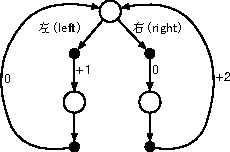
\includegraphics[width=.3\textwidth]{c3/img/exercise3-22.pdf}
\end{wrapfigure}
\mbox{}~
\begin{exer}
考虑如右图所示的持续式MDP. 顶部的状态中有唯一需要作出的决定, 其中可以采取两个动作, \textsf{left}以及\textsf{right}. 图中数字为采取动作后接收到的确定性奖赏. 仅有两个确定性的策略, $\pi_{\mathsf{left}}$与$\pi_{\mathsf{right}}$. 如果$\gamma = 0$的话哪个策略是最优的? 如果$\gamma = 0.9$呢? 或如果$\gamma = 0.5$呢?
\end{exer}

\begin{exer}
关于回收机器人, 给出针对$q_*$的贝尔曼方程.
\end{exer}

\begin{exer}
\figref{3.5}显示出, 在网格世界中, 最佳的状态的最优值为24.4(保留1位有效数字). 使用关于最优策略与\eqref{eq:3.8}的知识, 来用数学表达式表示这个值, 并将该值计算到3位有效数字. 
\end{exer}

\begin{exer}
给出一个使用$q_*$来表示$v_*$的等式.
\end{exer}

\begin{exer}
给出一个使用$v_*$与4参数函数$p$来表示$q_*$的等式.
\end{exer}

\begin{exer}
给出一个使用$q_*$来表示$\pi_*$的等式.
\end{exer}

\begin{exer}
给出一个使用$v_*$与4参数函数$p$来表示$\pi_*$的等式.
\end{exer}

\begin{exer}
使用3参数函数$p$\eqref{eq:3.4}以及2参数函数$r$, 来重写针对4种值函数($v_\pi$, $v_*$, $q_\pi$, $q_*$)的贝尔曼方程.
\end{exer}

% ----------------------------------- sec3.7 ---------------------------------------------
\section{最优性与近似}\label{sec:3.7}

我们已经定义了最优值函数与最优策略. 很明显, 学得了最优策略的代理将表现得非常好, 但在实际中这很少发生. 在我们所关心的各种问题中, 只有通过极端的计算开销才能获得最优策略. 对最优性的规范的见解, 可以帮助梳理本书中介绍的强化学习方法, 并为帮助我们理解各种学习算法的理论性质提供了一种途径, 但最优性仅是代理可以在不同程度上接近的一种理想化. 正如我们前面所讨论的, 即使我们拥有对环境的完整而准确的模型, 通过单纯地解贝尔曼最优性方程来得到最优策略通常是不现实的. 举个例子, 棋类游戏, 如国际象棋, 仅占到人类各种经验的极小的一部分, 但是规模庞大的定制计算机也无法计算出最优下法. 代理所面临的问题中极为关键的一个方面为其拥有多少算力, 更具体地说, 其能在一个时步中完成多少计算.

内存的大小也是一个重要的制约. 通常, 为了建立起对值函数、策略以及模型的估计, 通常需要大量的内存. 如果任务的状态集小而有限, 那么使用数组或表格<table>来进行估计是可行的, 其中各个状态(或状态-动作对)都有对应的表项. 我们将此称为\emph{表格式}情形, 并将对应的方法称为表格式方法. 而在我们感兴趣的许多实际情形下, 状态的数量太多了而远不能放入表格内. 在这种情形下, 我们必须使用某种简洁的参数化函数表示方法, 来对函数进行近似.

我们关于强化学习问题的框架迫使我们将就于使用近似. 然而, 其也为我们提供了独特机会用以达成合格近似. 例如, 在对近似求解最优动作时, 可能有很多状态代理遇到的概率非常小, 以至在这些状态上选择次优动作对代理接收到的奖赏总量几乎没有影响. 例如, Tesauro的西洋双陆棋程序拥有卓越的技巧, 哪怕其在面临不会在和高手的对战中出现的场景时, 有可能做出极糟糕的决策. 事实上, 极有可能TD-Gammon在游戏状态集的一大部分中都做出糟糕的决策. 强化学习的在线特性使得可以以这样的方式来近似最优策略: 在经常遇到的状态上投入更多的精力, 使得能在这些状态上做出好的决策——以在不常遇到的状态上投入更少精力为代价. 这是将强化学习同其他的近似求解MDP的方法区分开来的一个关键特性.

% ----------------------------------- sec3.8 ---------------------------------------------
\section{总结}\label{sec:3.8}

让我们总结下呈现在本章中的强化学习问题诸要素. 强化学习的目标从交互中学习如何决策以达成目的. 强化学习的\emph{代理}与其\emph{环境}在一系列离散的时步上交互. 两者接口间的具体细节定义出了具体的任务: \emph{动作}是需要由代理作出的选择; \emph{状态}为决策的基础; \emph{奖赏}是对做出的决策进行评估的基础. 代理内部的一切都为代理彻底知晓与控制; 而代理外部的一切可以被代理部分控制, 但为代理彻底知晓与否是不确定的. \emph{策略}为一概率性规则, 通过这个规则代理将动作作为状态的函数来进行选择. 代理的目标即为最大化随时间流逝所接收到的累积奖赏.

如果上述的强化学习设定与明确定义的转移概率一同表述, 那么就构成了\emph{马尔科夫决策过程}(MDP). 有限MDP为拥有有限状态集、有限动作集以及(于此处提出的)有限奖赏集的MDP. 当前强化学习的多数理论都限定于有限MDP, 但是这些方法与理念可以应用于更一般的情形.

\emph{回报}是未来的奖赏的函数, 也是代理寻求最大化的目标(从期望的角度). 取决于任务的特性以及我们是否希望对延迟的奖赏进行折扣, 其有数种不同的定义. 非折扣形式适合于\emph{分节式任务}, 在分节式任务中代理与环境间的交互可以自然地划分成不同的分节; 折扣形式适合于\emph{持续式任务}, 在持续式任务中交互不能自然地划分为不同的分节, 而是无限地持续下去. 我们希望统一两类任务中回报的定义, 使得同一套公式可以同时适用于分节式情形与连续式情形.

一策略的\emph{值函数}为每个状态(或状态-动作对)给出了在该策略下, 从该状态(或状态-动作对)起可以获得的期望回报. \emph{最优值函数}为每个状态(或状态-动作对)给出了各个策略中所能获得的最大期望回报. 值函数为最优的策略即为\emph{最优策略}. 对一个给定的MDP, 虽然针对状态或状态-动作对的最优值函数是唯一的, 但可能有多个最优策略. 任何就最优值函数而言贪心的策略一定是最优策略. \emph{贝尔曼最优性方程}为最优值函数必须满足的特殊一致性条件, 并且从理论上说, 我们可以从中解得最优值函数, 然后利用最优值函数我们可以相对轻松地确定最优策略.

取决于对代理起始时所拥有的关于环境的知识水平的不同假设, 强化学习问题可以以多种不同的方式呈现. 在有\emph{完全知识}的问题中, 代理有完整而准确的环境模型. 如果该环境为MDP, 那么模型应该包括4参数动态函数$p$\eqref{eq:3.2}. 而在\emph{不完全知识}的问题中, 无法获得完整且完美的环境模型.

即使代理有完整而准确的环境模型, 代理通常无法进行足够多的计算来彻底对其进行利用. 可以获得的内存的大小也是一个重要的制约因素. 我们可以需要内存来建立起对值函数、策略以及模型的准确估计. 在实际感兴趣的多数情形下, 状态通常太多了而无法放入表中, 此时必须进行函数近似.

对最优性的规范的见解, 可以帮助梳理本书中介绍的强化学习方法, 并为帮助我们理解各种学习算法的理论性质提供了一种途径, 但最优性仅是代理可以在不同程度上接近的一种理想化. 在强化学习中我们十分关心最优解不能被被找到, 但可以以某种方法被近似的情形. 

% ----------------------------------- bib ---------------------------------------------
\section*{参考文献与历史沿革}

暂不译

\printbibliography[title={参考文献}]

\end{document}